\documentclass[a4paper]{article}
\usepackage{vntex}
\usepackage{a4wide,amssymb,epsfig,latexsym,multicol,array,hhline,fancyhdr}
\usepackage{booktabs}
\usepackage{amsmath}
\usepackage{lastpage}
\usepackage[lined,boxed,commentsnumbered]{algorithm2e}
\usepackage{enumerate}
\usepackage{color}
\usepackage{graphicx}							% Standard graphics package
\usepackage{array}
\usepackage{tabularx, caption}
\usepackage{multirow}
\usepackage[framemethod=tikz]{mdframed}% For highlighting paragraph backgrounds
\usepackage{multicol}
\usepackage{rotating}
\usepackage{graphics}
\usepackage{geometry}
\usepackage{setspace}
\usepackage{epsfig}
\usepackage{tikz}
\usepackage{listings}
\usetikzlibrary{arrows,snakes,backgrounds}
\usepackage{hyperref}
\hypersetup{urlcolor=blue,linkcolor=black,citecolor=black,colorlinks=true} 
%\usepackage{pstcol} 								% PSTricks with the standard color package

\newtheorem{theorem}{{\bf Định lý}}
\newtheorem{property}{{\bf Tính chất}}
\newtheorem{proposition}{{\bf Mệnh đề}}
\newtheorem{corollary}[proposition]{{\bf Hệ quả}}
\newtheorem{lemma}[proposition]{{\bf Bổ đề}}

\everymath{\color{blue}}
%\usepackage{fancyhdr}
\setlength{\headheight}{40pt}
\pagestyle{fancy}
\fancyhead{} % clear all header fields
\fancyhead[L]{
 \begin{tabular}{rl}
    \begin{picture}(25,15)(0,0)
    \put(0,-8){
\includegraphics[width=8mm, height=8mm]{images/logoITSGUsmall.png}}
    %\put(0,-8){\epsfig{width=10mm,figure=hcmut.eps}}
   \end{picture}&
	%\includegraphics[width=8mm, height=8mm]{hcmut.png} & %
	\begin{tabular}{l}
		\textbf{\bf \ttfamily Trường Đại học Sài Gòn}\\
		\textbf{\bf \ttfamily Khoa Công Nghệ Thông Tin}
	\end{tabular} 	
 \end{tabular}
}
\fancyhead[R]{
	\begin{tabular}{l}
		\tiny \bf \\
		\tiny \bf 
	\end{tabular}  }
\fancyfoot{} % clear all footer fields
\fancyfoot[L]{\scriptsize \ttfamily Bài tập lớn môn Phát triển phần mềm mã nguồn mở - Niên khóa 2023-2024}
\fancyfoot[R]{\scriptsize \ttfamily Trang {\thepage}/\pageref{LastPage}}
\renewcommand{\headrulewidth}{0.3pt}
\renewcommand{\footrulewidth}{0.3pt}


%%%
\setcounter{secnumdepth}{4}
\setcounter{tocdepth}{3}
\makeatletter
\newcounter {subsubsubsection}[subsubsection]
\renewcommand\thesubsubsubsection{\thesubsubsection .\@alph\c@subsubsubsection}
\newcommand\subsubsubsection{\@startsection{subsubsubsection}{4}{\z@}%
                                     {-3.25ex\@plus -1ex \@minus -.2ex}%
                                     {1.5ex \@plus .2ex}%
                                     {\normalfont\normalsize\bfseries}}
\newcommand*\l@subsubsubsection{\@dottedtocline{3}{10.0em}{4.1em}}
\newcommand*{\subsubsubsectionmark}[1]{}
\makeatother

\definecolor{dkgreen}{rgb}{0,0.6,0}
\definecolor{gray}{rgb}{0.5,0.5,0.5}
\definecolor{mauve}{rgb}{0.58,0,0.82}

\lstset{frame=tb,
	language=Matlab,
	aboveskip=3mm,
	belowskip=3mm,
	showstringspaces=false,
	columns=flexible,
	basicstyle={\small\ttfamily},
	numbers=none,
	numberstyle=\tiny\color{gray},
	keywordstyle=\color{blue},
	commentstyle=\color{dkgreen},
	stringstyle=\color{mauve},
	breaklines=true,
	breakatwhitespace=true,
	tabsize=3,
	numbers=left,
	stepnumber=1,
	numbersep=1pt,    
	firstnumber=1,
	numberfirstline=true
}

\begin{document}

\begin{titlepage}
	\begin{center}
		TRƯỜNG ĐẠI HỌC SÀI GÒN \\
		KHOA CÔNG NGHỆ THÔNG TIN
	\end{center}
	\vspace{1cm}

	\begin{figure}[h!]
		\begin{center}
			
\includegraphics[width=3cm]{images/logoITSGU.png}
		\end{center}
	\end{figure}

	\vspace{1cm}


	\begin{center}
		\begin{tabular}{c}
			\multicolumn{1}{l}{\textbf{{\Large PHÁT TRIỂN PHẦN MỀM MÃ NGUỒN MỞ}}} \\
			~~                                                                    \\
			\hline
			\\
			\multicolumn{1}{l}{\textbf{{\Large Xây dựng phần mềm}}}               \\
			\\

			\textbf{{\Large HarmonyHub - Ứng dụng nghe nhạc trên PYTHON}}         \\
			\\
			\hline
		\end{tabular}
	\end{center}

	\vspace{3cm}

	\begin{table}[h]
		\begin{tabular}{rrl}
			\hspace{5 cm} & GVHD: & Từ Lãng Phiêu                     \\
			              & SV:   & Nguyễn Anh Danh - 3121410103      \\
			              &       & Phan Duy - 3121410003             \\
			              &       & Văn Phú Hiếu - 3121410201         \\
			              &       & Đỗ Nguyễn Hoàng Tuấn - 3121410554 \\
			% & & SV3 - MSSV \\
			% & & SV4 - MSSV\\
		\end{tabular}
		\vspace{1.5 cm}
	\end{table}

	\begin{center}

		{\footnotesize TP. HỒ CHÍ MINH, THÁNG 5/2024}
	\end{center}
\end{titlepage}


\thispagestyle{empty}
\newpage
\begin{center}
	\section*{Nhận xét, đánh giá của giảng viên}
\end{center}
\begin{flushleft}
	\dotfill
\end{flushleft}
\begin{flushleft}
	\dotfill
\end{flushleft}
\begin{flushleft}
	\dotfill
\end{flushleft}
\begin{flushleft}
	\dotfill
\end{flushleft}
\begin{flushleft}
	\dotfill
\end{flushleft}
\begin{flushleft}
	\dotfill
\end{flushleft}
\begin{flushleft}
	\dotfill
\end{flushleft}
\begin{flushleft}
	\dotfill
\end{flushleft}
\begin{flushleft}
	\dotfill
\end{flushleft}
\begin{flushleft}
	\dotfill
\end{flushleft}
\begin{flushleft}
	\dotfill
\end{flushleft}
\begin{flushleft}
	\dotfill
\end{flushleft}
\begin{flushleft}
	\dotfill
\end{flushleft}
\begin{flushleft}
	\dotfill
\end{flushleft}
\begin{flushleft}
	\dotfill
\end{flushleft}
\begin{flushleft}
	\dotfill
\end{flushleft}
\begin{flushleft}
	\dotfill
\end{flushleft}
\begin{flushleft}
	\dotfill
\end{flushleft}
\begin{flushleft}
	\dotfill
\end{flushleft}
\begin{flushleft}
	\dotfill
\end{flushleft}
\begin{flushleft}
	\dotfill
\end{flushleft}
\begin{flushleft}
	\dotfill
\end{flushleft}
\begin{flushleft}
	\dotfill
\end{flushleft}
\begin{flushleft}
	\dotfill
\end{flushleft}
\begin{flushleft}
	\dotfill
\end{flushleft}
\begin{flushleft}
	\dotfill
\end{flushleft}
%%%%%%%%%%%%%%%%%%%%%%%%%%%%%%%%%


%%%%%%%%%%%%%%%%%%%%%%%%%%%%%%%%%
\newpage
\begin{center}
	\section*{Lời cảm ơn}
\end{center}
\begin{flushleft}
	Chúng em xin gửi lời cảm ơn chân thành nhất đối với các thầy cô ở khoa Công Nghệ Thông Tin, trường Đại học Sài Gòn đã tạo điều kiện cho chúng em tiếp cận và tìm hiểu để hoàn thành đồ án môn học lần này. Và chúng em cũng xin chân thành cảm ơn thầy Từ Lãng Phiêu giáo viên giảng dạy đã nhiệt tình hướng dẫn chúng em hoàn thành đồ án lần này.
	Trong quá trình thực hiện nghiên cứu và thực hiện làm báo cáo đồ án, do kinh nghiệm thực tế chưa được nhiều, nên bài báo cáo của chúng em có thể vẫn còn những thiếu sót và chưa được hoàn chỉnh nên mong rằng chúng em sẽ nhận được những đóng góp ý kiến đóng góp bổ ích từ thầy để chúng em có thể khắc phục cho những bài báo cáo sau.

\end{flushleft}
\begin{flushright}
	\text{Chúng em xin trân trọng cảm ơn thầy!}
\end{flushright}

\newpage
\tableofcontents
\newpage

%%%%%%%%%%%%%%%%%%%%%%%%%%%%%%%%%


%%%%%%%%%%%%%%%%%%%%%%%%%%%%%%%%%
\section{Phần 1: Mở đầu}
\subsection{Lý do chọn đề tài}

Công nghệ thông tin ngày càng trở thành một phần không thể thiếu trong cuộc sống hiện đại, và ngôn ngữ lập trình Python đã và đang đóng một vai trò quan trọng trong việc phát triển các ứng dụng công nghệ thông tin. Python với cấu trúc rõ ràng, dễ đọc và dễ học, đã trở thành một trong những lựa chọn hàng đầu cho nhiều lập trình viên trên toàn thế giới.

Âm nhạc là một phần quan trọng của cuộc sống, mang lại niềm vui, sự thư giãn và là nguồn cảm hứng cho con người. Với sự phát triển của công nghệ, việc nghe nhạc đã trở nên dễ dàng hơn bao giờ hết. Tuy nhiên, việc tìm kiếm một ứng dụng nghe nhạc phù hợp với nhu cầu cá nhân không phải lúc nào cũng dễ dàng.

Chính vì vậy, chúng em đã chọn đề tài "Phát triển ứng dụng nghe nhạc sử dụng ngôn ngữ Python". Mục tiêu của chúng em là tạo ra một ứng dụng nghe nhạc đơn giản nhưng đầy đủ tính năng, dễ sử dụng và có thể tùy chỉnh theo nhu cầu của người dùng. Chúng em tin rằng, với sự linh hoạt và mạnh mẽ của Python, chúng em có thể đạt được mục tiêu này.

% \begin{mdframed}[hidealllines=true,backgroundcolor=magenta!10]
% 	\begin{lstlisting}
% 		% ------------------------------- %
% 		%     XOA MAN HINH VA CAC BIEN    %
% 		% ------------------------------- %
% 		clear
% 		clc

% 		% ------------------------------- %
% 		%      NHAP DU LIEU BAI TOAN      %
% 		% ------------------------------- %
% 		n = ...;      % So nguoi dan
% 		m = ...;      % So benh vien
% 		% Ma tran D bieu dien thu tu uu tien cua benh vien doi voi benh nhan
% 		% ung voi tung hang
% 		D = [...];
% 		% Ma tran B bieu dien thu tu uu tien cua benh nhan doi voi benh vien
% 		% ung voi tung cot
% 		B = [...];
% 		% Ma tran c bieu dien suc chua cua tung benh vien
% 		c = [...];
% 		% Ma tran a bieu dien moi benh nhan chi duoc chon lua mot benh vien
% 		a = ones(n,1);

% 		% ------------------------------- %
% 		% GIAI BAI TOAN BANG SOLVER MOSEK %
% 		% ------------------------------- %
% 		cvx_begin
% 			cvx_solver mosek
% 			% Bien x(i,j) chi nhan gia tri 0 hoac 1
% 			% ung voi su ghep goi benh nhan r_i voi benh vien h_j
% 			variable x(n,m) binary
% 			% Toi da tong cac bien x(i,j)
% 			% tuc la cang nhieu cap duoc ghep doi cang tot
% 			maximize( 0 )
% 			subject to
% 				% Tong cac hang trong cung mot cot (so benh nhan duoc chon)
% 				% nho hon hoac bang suc chua cua benh vien
% 				sum(x,1) <= c;
% 				% Tong cac cot trong cung mot cot (so benh vien duoc chon)
% 				% nho hon hoac bang 1
% 				sum(x,2) <= a;
% 			% Bao dam khong co cac cap chan
% 			for u = 1:n
% 				for v = 1:m
% 					%Tinh so hang dau tien trong ham dieu kien on dinh
% 					t1 = 0;
% 					for j = 1:m 
% 						t1 = t1 + lt(D(u,j),D(u,v)) * x(u,j); 
% 					end
% 					%Tinh so hang thu hai trong ham dieu kien on dinh
% 					t2 = 0;
% 					for i = 1:n
% 						t2 = t2 + lt(B(i,v),B(u,v)) * x(i,v) / c(v); 
% 					end
% 					%Xac lap ham dieu kien on dinh
% 					t1 + t2 + x(u,v) >= 1;
% 					%Ham dam bao cac cap (r_u,h_v) duoc xet nam trong A, neu
% 					%cap do khong nam trong A thi x_uv = 0
% 					if D(u,v) == m+n+1 || B(u,v) == m+n+1
% 						(eq(D(u,v),m+n+1) + eq(B(u,v),m+n+1)) * x(u,v) == 0;
% 					end
% 				end
% 			end
% 		cvx_end

% 		% ------------------------------- %
% 		%  HIEN THI KET QUA RA MAN HINH   %
% 		% ------------------------------- %
% 		D
% 		B
% 		c
% 		x       % Cac cap duoc ghep doi
% 	\end{lstlisting}
% \end{mdframed}
\subsection{Mục đích - mục tiêu của đề tài}
\textbf{-Mục đích}
\begin{itemize}
	\item Nắm chắc được kỹ năng và kiến thức về ngôn ngữ lập trình Python.
	\item Tìm hiểu về cách thức hoạt động của một ứng dụng nghe nhạc.
	\item Tìm hiểu về thư viện Pygame, MySQL Connector, \dots
	\item Cũng cố, áp dụng, nâng cao kiến thức đã học.
\end{itemize}
\textbf{-Mục tiêu}
\begin{itemize}
	\item Vận dụng được tính chất của lập trình hướng đối tượng.
	\item Xây dựng một ứng dụng nghe nhạc đơn giản, dễ sử dụng.
\end{itemize}
\subsection{Phạm vi đề tài}
\begin{itemize}
	\item Ứng dụng có thể tìm kiếm, phát nhạc từ cơ sở dữ liệu.
	\item Ứng dụng có thể tạo danh sách phát, tạo playlist.
\end{itemize}
\subsection{Nội dung đề tài}
\begin{flushleft}
	Bao gồm 2 phần:
	\begin{itemize}
		\item Phần 1: Mở đầu
		\item Phần 2: Thực hiện ứng dụng nghe nhạc trên Python
		      \begin{itemize}
			      \item Mở đầu
			      \item Xây dựng ứng dụng nghe nhạc bằng cách sử dụng các thư viện của Python:
			            \begin{itemize}
				            \item Phân tích yêu cầu
				            \item Thiết kế kiến trúc
				            \item Thiết kế cơ sở dữ liệu
				            \item Xây dựng chức năng
				            \item Kiểm thử và sửa lỗi
			            \end{itemize}
		      \end{itemize}
	\end{itemize}
\end{flushleft}

\section{Xây dựng ứng dụng nghe nhạc trên Python bằng các thư viện của Python}
\subsection{Đôi nét về ứng dụng nghe nhạc}
\begin{flushleft}
	-Ứng dụng nghe nhạc không chỉ là một công cụ giúp người dùng tìm kiếm và phát nhạc từ cơ sở dữ liệu. Nó còn là một nền tảng giúp người dùng trải nghiệm âm nhạc theo cách riêng của họ.

	-Tìm kiếm và phát nhạc: Ứng dụng nghe nhạc cho phép người dùng tìm kiếm bài hát, album, nghệ sĩ yêu thích của họ từ một cơ sở dữ liệu lớn. Người dùng có thể phát nhạc trực tiếp từ ứng dụng, điều chỉnh âm lượng, chọn chế độ phát (như phát lại, lặp lại, ngẫu nhiên), và xem thông tin chi tiết về bài hát đang phát.

	-Tạo danh sách phát: Người dùng có thể tạo danh sách phát cá nhân, thêm bài hát vào danh sách phát, sắp xếp thứ tự các bài hát trong danh sách phát, và chia sẻ danh sách phát với bạn bè. Điều này giúp người dùng tổ chức bộ sưu tập âm nhạc của họ theo cách mà họ muốn.

	-Tạo playlist: Playlist là một tính năng mạnh mẽ giúp người dùng tổ chức và phát nhạc theo chủ đề, tâm trạng, hoặc sự kiện. Người dùng có thể tạo playlist, thêm bài hát vào playlist, và chia sẻ playlist với cộng đồng.

	-Khám phá âm nhạc mới: Ứng dụng nghe nhạc thường có tính năng khám phá, giúp người dùng tìm kiếm và khám phá âm nhạc mới dựa trên sở thích âm nhạc của họ. Điều này giúp người dùng mở rộng bộ sưu tập âm nhạc của họ và khám phá những nghệ sĩ, thể loại mới.

	-Như vậy, ứng dụng nghe nhạc không chỉ giúp người dùng nghe nhạc, mà còn giúp họ trải nghiệm âm nhạc theo cách riêng của họ, khám phá âm nhạc mới, và chia sẻ niềm đam mê âm nhạc với cộng đồng. Đây chính là lý do mà việc phát triển ứng dụng nghe nhạc sử dụng Python trở nên hấp dẫn và thú vị. Python với khả năng mạnh mẽ và linh hoạt của mình, cho phép chúng ta tạo ra những ứng dụng nghe nhạc phong phú và đa dạng, phục vụ cho nhu cầu ngày càng đa dạng của người dùng.

\end{flushleft}
\subsection{Tổng quan và phân tích}
\subsubsection{Khảo sát}
\begin{flushleft}
	-Ứng dụng nghe nhạc là một nền tảng trực tuyến phổ biến, đặc biệt trong cộng đồng người yêu âm nhạc và các nhóm cộng đồng trực tuyến khác.
	Một trong những lợi ích của ứng dụng nghe nhạc là tính linh hoạt và đa dạng của nó. Người dùng có thể tùy chỉnh các danh sách phát và quyền truy cập cho từng bài hát,
	tạo ra các thể loại khác nhau để quản lý bộ sưu tập âm nhạc và tùy chỉnh các cài đặt âm thanh cho phù hợp với nhu cầu của mình.

	-Việc tạo ứng dụng nghe nhạc cũng là một lợi ích lớn, giúp việc quản lý bộ sưu tập âm nhạc trở nên dễ dàng hơn và giảm thiểu
	thời gian và công sức cho các hoạt động quản lý. Ứng dụng có thể tự động thực hiện các nhiệm vụ như kiểm tra và cập nhật thông tin bài hát,
	quản lý danh sách phát và nhiều tính năng khác \dots

	-Tuy nhiên, ứng dụng nghe nhạc cũng có một số hạn chế như việc không thể tùy chỉnh giao diện của ứng dụng hoặc các danh sách phát quá nhiều.
\end{flushleft}
\subsubsection{Phân tích}
\begin{table}[h]
	\centering
	\begin{tabular}{|l|p{10cm}|}
		\hline
		\textbf{Thư viện} & \textbf{Mô tả}                                                                                                                                                                                                                                                                                                                                                      \\
		\hline
		mysql.connector   & Thư viện mysql.connector trong Python cung cấp các hàm để tương tác với cơ sở dữ liệu MySQL. Cho phép tạo ra các ứng dụng có khả năng tương tác mạnh mẽ với cơ sở dữ liệu, thực hiện các tác vụ như truy vấn, cập nhật, và quản lý dữ liệu. Thư viện mysql.connector giúp lập trình viên tạo ra các ứng dụng có khả năng tương tác mạnh mẽ với cơ sở dữ liệu MySQL. \\
		\hline
		pygame            & Thư viện pygame trong Python cung cấp các hàm để tạo ra các ứng dụng đồ họa, bao gồm các trò chơi và các ứng dụng đa phương tiện khác. Tạo ra các ứng dụng có đồ họa mạnh mẽ, tương tác với người dùng qua các sự kiện đầu vào, và tạo ra các hiệu ứng âm thanh và hình ảnh. Thư viện pygame giúp lập trình viên tạo ra các ứng dụng đồ họa mạnh mẽ và tương tác.   \\
		\hline
		tkinter           & Thư viện tkenter trong Python cung cấp các hàm để tạo ra các ứng dụng đồ họa, các ứng dụng đa phương tiện khác. Tạo ra các ứng dụng có đồ họa mạnh mẽ, tương tác với người dùng qua các sự kiện đầu vào, và tạo ra các hiệu ứng âm thanh và hình ảnh.                                                                                                               \\
		\hline
		PIL               & Thư viện này cung cấp hỗ trợ định dạng tệp phong phú, hiệu quả và khả năng xử lý hình ảnh mạnh mẽ.                                                                                                                                                                                                                                                                  \\
		\hline
	\end{tabular}
	\caption{Các thư viện Python được sử dụng cho việc phát triển ứng dụng}
	\label{tab:my_label}
\end{table}
%%%%%%%%%%%%%%%%%%%%%%%%%%%%%%%%%
\clearpage
\newpage
\subsection{Xây dựng ứng dụng nghe nhạc}
\subsubsection{Cài đặt các thư viện cần thiết}
\begin{flushleft}
	-Visual Studio Code (64-bit).

	-Điều đầu tiên cần làm để lập trình ứng dụng nghe nhạc trên Python là cài đặt các thư viện cần thiết.
	Các thư viện này giúp chúng ta tương tác với hệ thống, tạo ra các ứng dụng đa luồng,
	tương tác với cơ sở dữ liệu, và tạo ra các ứng dụng đồ họa mạnh mẽ.

	Sau đó hệ thống sẽ tự động cài đặt các thư viện cần thiết:
	\begin{figure}[h]
		\centering
		\includegraphics[width=\textwidth]{images/Hình2-Libary.png}
		\caption{Cài đặt thư viện MySQL}
	\end{figure}
	\begin{figure}[h]
		\centering
		\includegraphics[width=\textwidth]{images/Hình3-Libary.png}
		\caption{Cài đặt thư viện Pygame (Do đã cài đặt nên ta sẽ không cần cài nữa)}
	\end{figure}
\end{flushleft}
\subsection{Các bước khởi tạo ứng dụng nghe nhạc}
\subsubsection{Khai báo thư viện}
\begin{flushleft}
	Sau khi cài đặt các thư viện cần thiết, ta tiến hành khai báo các thư viện cần dùng:
	\begin{figure}[h]
		\centering
		\includegraphics[width=\textwidth]{images/Hình4-Libary.png}
		\includegraphics{images/Hình5-Libary.png}
		\caption{Khai báo thư viện}
	\end{figure}
\end{flushleft}
\newpage
\subsection{Sơ đồ cơ sở dữ liệu}
\begin{flushleft}
	-Để lưu trữ thông tin về bài hát, album, nghệ sĩ, và các thông tin khác, chúng ta cần tạo một cơ sở dữ liệu.

	-Chúng ta đồng thời sẽ sử dụng XAMPP để tạo cơ sở dữ liệu MySQL và thiết kế cơ sở dữ liệu cho ứng dụng trên đó.

	-Chúng ta có sơ đồ cơ sở dữ liệu như sau:
	\begin{figure}[h]
		\begin{center}
			\includegraphics[width=\textwidth]{images/Hình4-DB.png}
			\caption{Sơ đồ cơ sở dữ liệu cho ứng dụng nghe nhạc}
		\end{center}
	\end{figure}

	-Sau khi chúng ta đã có sơ đồ cơ sở dữ liệu, chúng ta sẽ tiến hành kết nối cơ sở dữ liệu với ứng dụng thông qua thư viện MySQL Connector
	và thực hiện các thao tác truy vấn, cập nhật dữ liệu từ cơ sở dữ liệu.

	\begin{figure}
		\centering
		\includegraphics[width=\textwidth]{images/Hình7-ConnectDB.png}
		\caption{Khai báo thư viện và kết nối cơ sở dữ liệu thông qua class ConnectDB.py}
		\begin{flushleft}
			-Giải thích:

			+Class ConnectDB chứa hàm khởi tạo và hàm kết nối cơ sở dữ liệu gồm các thông số sau:
			\begin{itemize}
				\item host: địa chỉ IP của máy chủ cơ sở dữ liệu.
				\item user: tên người dùng để truy cập cơ sở dữ liệu.
				\item password: mật khẩu để truy cập cơ sở dữ liệu.
				\item database: tên cơ sở dữ liệu.
			\end{itemize}

			+Nếu kết nối thành công, hàm kết nối sẽ trả về một đối tượng connection, ngược lại sẽ trả về None.
		\end{flushleft}
	\end{figure}

\end{flushleft}
\clearpage
\newpage
\subsection{Kiến trúc ứng dụng}
\begin{flushleft}
	-Về kiến trúc thiết kế mô hình phát triển ứng dụng nghe nhạc, chúng ta sẽ sử dụng mô hình 3 lớp (3-tier architecture)
	bao gồm 3 lớp chính: DAL, BLL, và GUI.
	\begin{figure}[h]
		\centering
		\includegraphics{images/Hình8-Architecture.png}
		\caption{Kiến trúc ứng dụng nghe nhạc}
	\end{figure}
\end{flushleft}

\subsection{Xây dựng chức năng}
\begin{flushleft}
	-Để xây dựng chức năng cho ứng dụng nghe nhạc, chúng ta sẽ tạo ra các class đối tượng (Object) tương ứng với các bảng trong cơ sở dữ liệu ở thư mục DTO (Data Transfer Object):
	\begin{figure}[h]
		\centering
		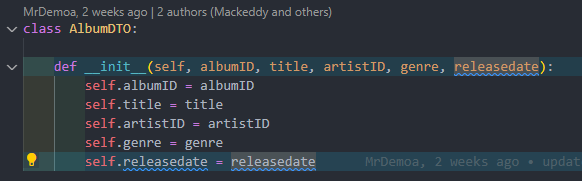
\includegraphics[width=\textwidth]{images/AlbumDTO.png}
	\end{figure}
\end{flushleft}
\begin{flushleft}
	\begin{figure}[h]
		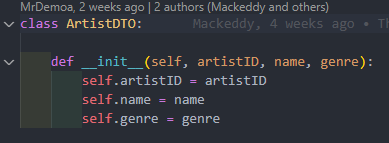
\includegraphics[width=\textwidth]{images/ArtistDTO.png}
		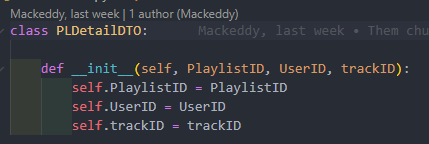
\includegraphics[width=\textwidth]{images/PlayListDetailDTO.png}
		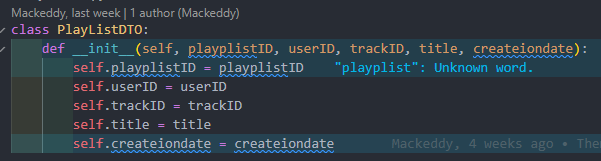
\includegraphics[width=\textwidth]{images/PlayListDTO.png}
		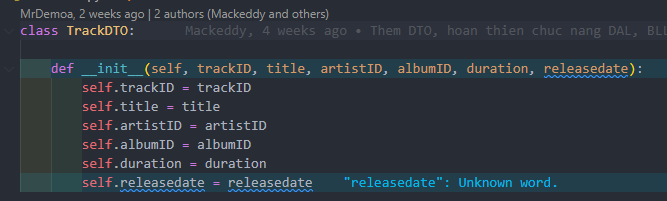
\includegraphics[width=\textwidth]{images/TrackDTO.png}
	\end{figure}
\end{flushleft}
\clearpage

\newpage
\begin{flushleft}
	\begin{figure}[h]
		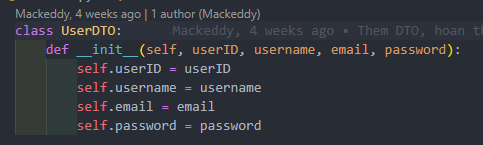
\includegraphics[width=\textwidth]{images/UserDTO.png}
		\caption{Các class DTO}
	\end{figure}
	-Sau khi chúng ta đã tạo các class DTO, chúng ta sẽ tiến hành tạo các class ở tầng DAL (Data Access Layer) để thực hiện các thao tác truy vấn, cập nhật dữ liệu từ cơ sở dữ liệu:
\end{flushleft}
\begin{figure}[h]
	\centering
	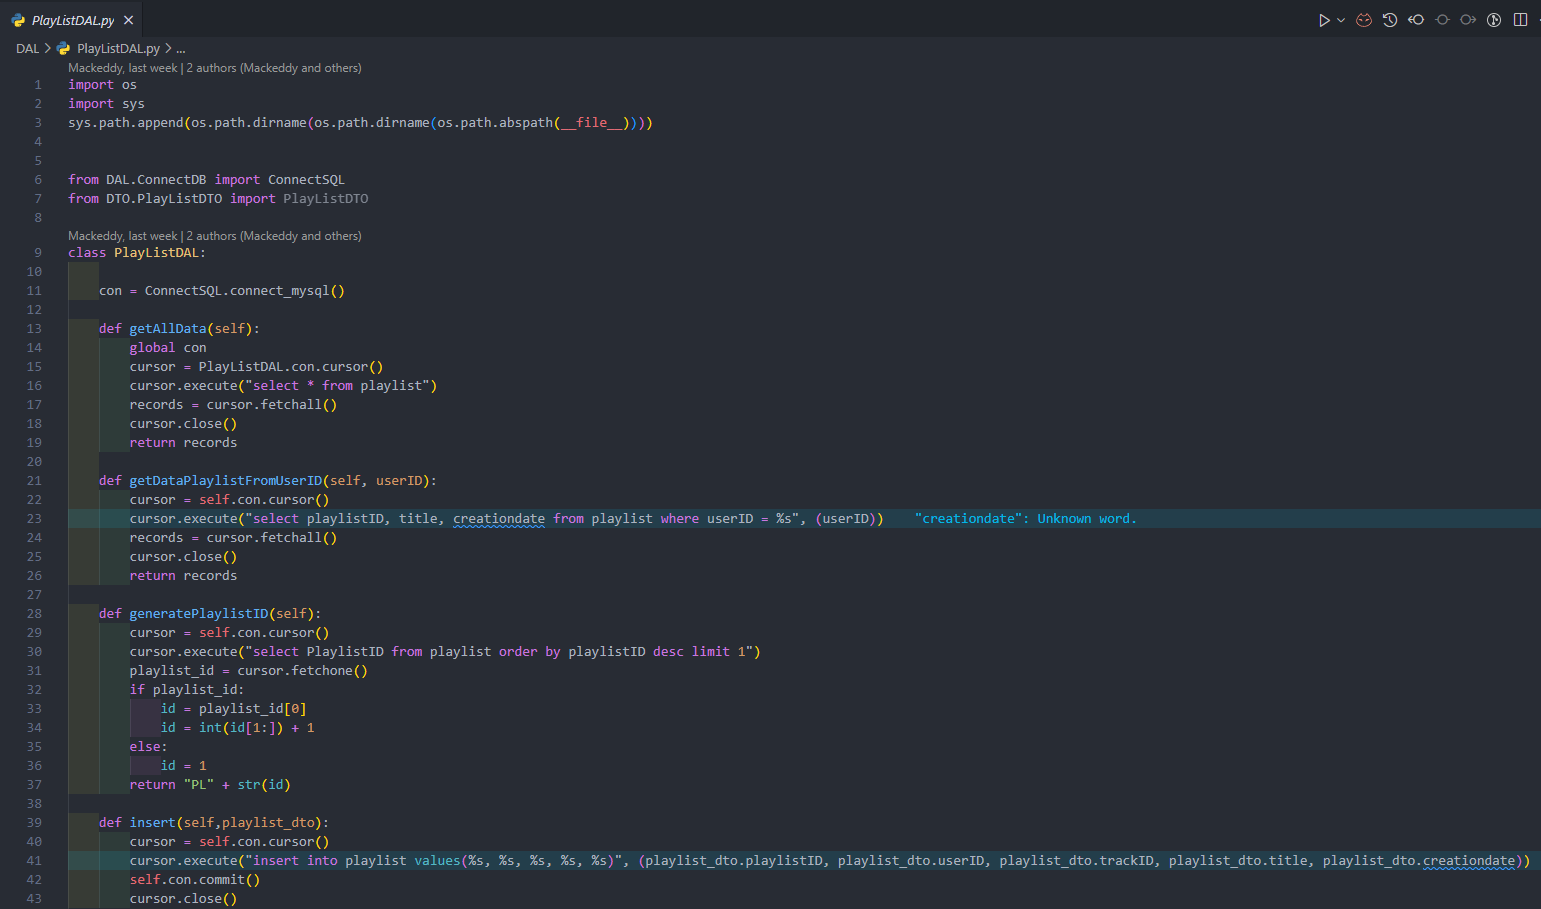
\includegraphics[width=\textwidth]{images/PlaylistDAL-1.png}
\end{figure}
\clearpage

\newpage
\begin{figure}
	\includegraphics[width=\textwidth]{images/PlaylistDAL-2.png}
	\caption{Code cho class PlaylistDAL gồm các phương thức CRUD (Create, Read, Update, Delete)}
\end{figure}

\begin{flushleft}
	-Giải thích:
	\begin{itemize}
		\item Phương thức \textbf{getAllData(self)} trả về danh sách tất cả các playlist trong cơ sở dữ liệu.
		      \begin{flushleft}
			      +Chi tiết hơn:

			      -Đầu tiên, ta sẽ thiết lập kết nối đến cơ sở dữ liệu thông qua class ConnectDB.

			      -Sau đó, ta sẽ tạo 1 cursor để thực hiện các thao tác truy vấn dữ liệu.

			      -Cuối cùng, ta sẽ thực hiện truy vấn dữ liệu và trả về kết quả lưu về records
		      \end{flushleft}
		\item Phương thức \textbf{getPlaylistIDByUserID(self, userID)} trả về danh sách playlist dựa vào id của user.
		      \begin{flushleft}
			      +Chi tiết hơn:

			      -Đầu tiên, ta sẽ thiết lập kết nối đến cơ sở dữ liệu.

			      -Sau đó, ta sẽ tạo 1 cursor để thực hiện các thao tác truy vấn dữ liệu và lấy ra toàn bộ playlist dựa vào id của user.

			      -Cuối cùng, ta sẽ thực hiện truy vấn dữ liệu và trả về kết quả lưu về records (trong trường hợp này, ta sẽ truy vấn dữ liệu dựa vào id của user).
		      \end{flushleft}
		\item Phương thức \textbf{getDataPlayListFromUserId(self, userID)} trả về thông tin chi tiết của một playlist dựa vào id.
		      \begin{flushleft}
			      +Chi tiết hơn:

			      -Đầu tiên, ta sẽ thiết lập kết nối đến cơ sở dữ liệu thông qua class ConnectDB.

			      -Sau đó, ta sẽ tạo 1 cursor để thực hiện các thao tác truy vấn dữ liệu.

			      -Cuối cùng, ta sẽ thực hiện truy vấn dữ liệu và trả về kết quả lưu về records (trong trường hợp này, ta sẽ truy vấn dữ liệu dựa vào id của user).
		      \end{flushleft}
		\item Phương thức \textbf{generatePlayListID(self)} tạo một ID duy nhất cho playlist mới.
		      \begin{flushleft}
			      +Chi tiết hơn:

			      -Đầu tiên, ta sẽ thiết lập kết nối đến cơ sở dữ liệu thông qua class ConnectDB.

			      -Sau đó, ta sẽ tạo 1 cursor để thực hiện các thao tác truy vấn dữ liệu.

			      -Lấy ra kết quả đầu tiên của query, kiểm tra xem nếu nó tồn tại thì
			      lấy ID đó, loại bỏ ký tự đầu tiên (giả sử là 'PL'), chuyển phần còn lại thành số và cộng thêm một.
			      Điều này đảm bảo rằng mỗi playlist có một ID duy nhất.

			      Nếu không nhận được ID trả về, điều đó có nghĩa là chưa có playlist nào trong cơ sở dữ liệu.
			      Vì vậy, nó đơn giản là đặt ID cho playlist mới là 1.

			      Cuối cùng, nó thêm 'PL' vào đầu ID (để chỉ ra rằng đó là Playlist ID) và trả về nó.
			      Đây sẽ là ID duy nhất cho playlist mới.
		      \end{flushleft}
		\item Phương thức \textbf{insert(self, playlist\_dto)} thêm một playlist mới vào cơ sở dữ liệu.
		      \begin{flushleft}
			      +Chi tiết hơn:

			      -Đầu tiên, ta sẽ thiết lập kết nối đến cơ sở dữ liệu thông qua class ConnectDB.

			      -Sau đó, ta sẽ tạo 1 cursor để thực hiện các thao tác truy vấn dữ liệu.

			      -Sau khi chuẩn bị xong câu lệnh, nó được thực thi bằng cách sử dụng con trỏ (Cursor). Điều này thêm playlist mới vào cơ sở dữ liệu.

			      -Tuy nhiên, chỉ thực thi câu lệnh không đủ. Các thay đổi cần được lưu lại. Đó là lý do tại sao self.con.commit() được sử dụng - nó lưu lại bất kỳ thay đổi nào được thực hiện kể từ lần cuối cùng thay đổi được lưu lại.

			      -Cuối cùng, con trỏ được đóng. Điều này được thực hiện khi chúng ta đã hoàn thành với nó, để giải phóng tài nguyên.
		      \end{flushleft}
		\item Phương thức \textbf{deletePlayList(playlistID)} xóa một playlist dựa vào id.
		      \begin{flushleft}
			      +Chi tiết hơn:

			      -Đầu tiên, ta thiết lập kết nối và tạo con trỏ (Cursor).

			      -Sau đó, ta thực thi câu lệnh DELETE để xóa playlist dựa vào id và đếm số lượng dòng bị ảnh hưởng.

			      -Nếu số lượng dòng bị ảnh hưởng lớn hơn 0, điều đó có nghĩa là playlist đã được xóa thành công.

			      -Cuối cùng, ta lưu lại các thay đổi và đóng con trỏ.
		      \end{flushleft}
		\item Phương thức \textbf{updatePlayList(playlist\_dto)} cập nhật thông tin của một playlist.
		      \begin{flushleft}
			      +Cách thức hoạt động tương tự như phương thức insert, nhưng thay vì thêm mới, nó sẽ cập nhật thông tin của playlist đã tồn tại.
		      \end{flushleft}
	\end{itemize}
\end{flushleft}

\clearpage
\newpage
\begin{figure}[h]
	\centering
	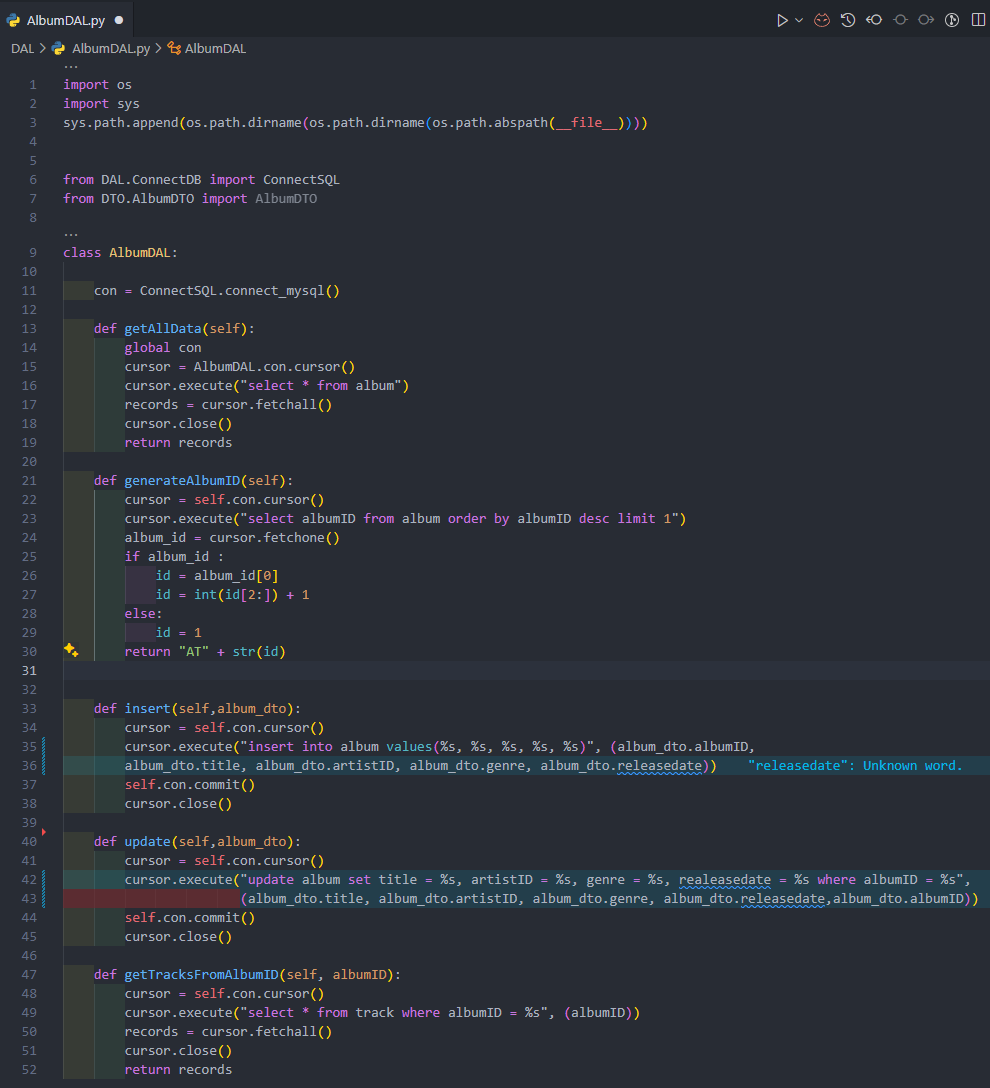
\includegraphics[width=0.9\textwidth]{images/albumDAL.png}
	\caption{Code cho class AlbumDAL gồm các phương thức đọc, thêm, sửa}
\end{figure}

\begin{flushleft}
	-Giải thích:
	\begin{itemize}
		\item Phương thức \textbf{getAllData(self)} trả về danh sách tất cả các album trong cơ sở dữ liệu.
		      \begin{flushleft}
			      + Tương tự như PlayListDAL chỉ khác là trả về danh sách album.
		      \end{flushleft}
		\item Phương thức \textbf{generateAlbumID(self, albumID)} tạo một ID duy nhất cho album mới.
		      \begin{flushleft}
			      +Chi tiết hơn:

			      -Đầu tiên, chúng ta thiết lập kết nối với cơ sở dữ liệu.

			      -Sau đó, chúng ta yêu cầu cơ sở dữ liệu trả về ID của album được thêm gần đây nhất. Chúng ta làm điều này bằng cách chạy một lệnh yêu cầu "cho tôi albumID từ bảng album, nhưng hãy đảm bảo rằng bạn đưa cho tôi cái cuối cùng bạn có".

			      -Bây giờ, có hai khả năng: hoặc chúng ta nhận được một ID trả về, hoặc không. Nếu chúng ta nhận được một ID, điều đó có nghĩa là đã có một số album trong cơ sở dữ liệu. Vì vậy, chúng ta lấy ID đó, loại bỏ hai ký tự đầu tiên (giả sử là 'AT'), chuyển phần còn lại thành một số và cộng thêm một vào nó. Điều này đảm bảo rằng mỗi album có một ID duy nhất.

			      -Nếu chúng ta không nhận được ID trả về, điều đó có nghĩa là chưa có album nào trong cơ sở dữ liệu. Vì vậy, chúng ta đơn giản là đặt ID cho album mới là 1.

			      -Cuối cùng, chúng ta thêm 'AT' vào đầu ID (để chỉ ra rằng đó là Album ID), và trả về nó. Đây sẽ là ID duy nhất cho album mới.
		      \end{flushleft}
		\item Phương thức \textbf{insert(self, album\_dto)} tạo một album mới trong cơ sở dữ liệu.
		      \begin{flushleft}
			      +Tương tự như hàm insert của PlayListDAL chỉ khác là thêm mới album.
		      \end{flushleft}
		\item Phương thức \textbf{update(album\_dto)} sửa thông tin của một album.
		      \begin{flushleft}
			      +Tương tự như hàm update của PlayListDAL chỉ khác là sửa album.
		      \end{flushleft}
		\item Phương thức \textbf{getTracksFromAlbumID(self, albumID)} lấy ra danh sách các bài hát theo albumID.
		      \begin{flushleft}
			      +Tương tự như hàm getDataPlayListFromUserId của PlayListDAL chỉ khác là lấy ra danh sách bài hát theo albumID.
		      \end{flushleft}
	\end{itemize}
\end{flushleft}
\clearpage

\newpage
\begin{figure}[h]
	\centering
	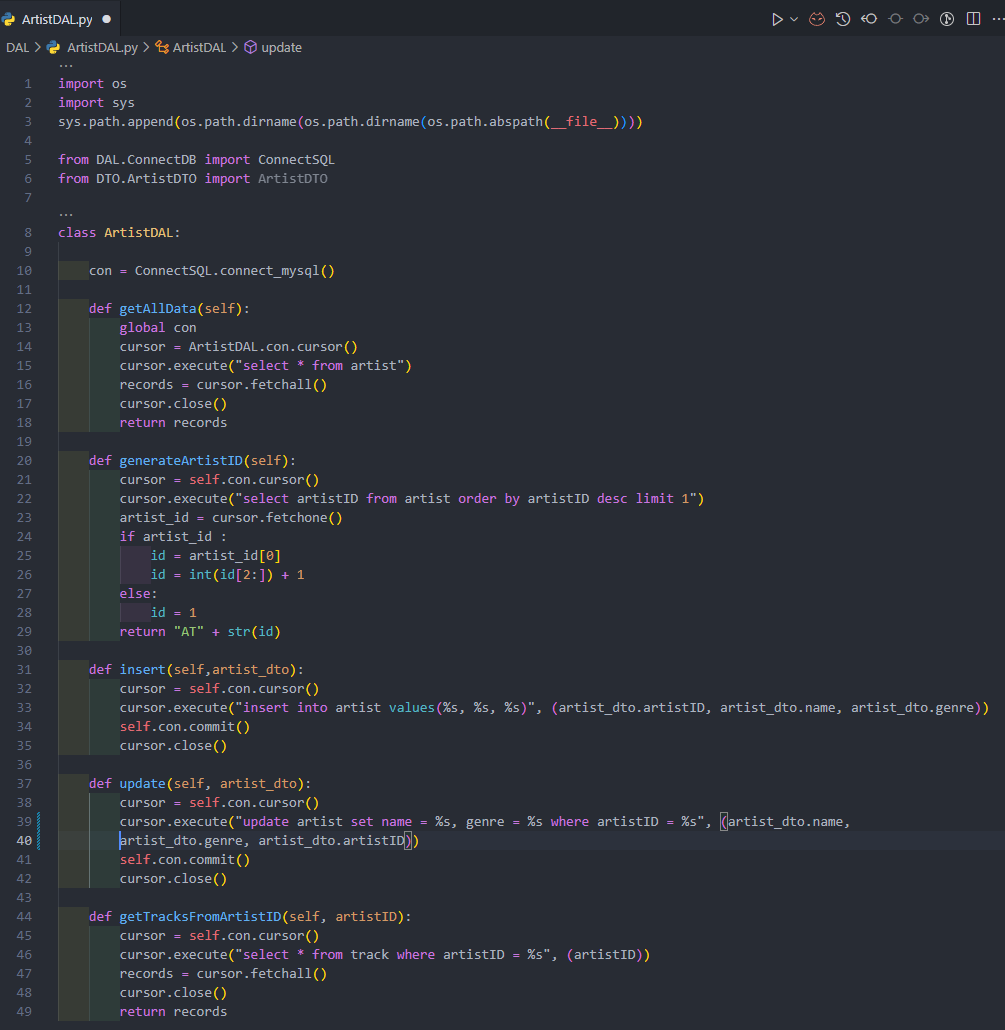
\includegraphics[width=\textwidth]{images/artistDAL.png}
	\caption{Code cho class ArtistDAL gồm các phương thức đọc, thêm, sửa}
\end{figure}
\begin{flushleft}
	-Giải thích:
	\begin{itemize}
		\item Phương thức \textbf{getAllData(self)} trả về danh sách tất cả các nghệ sĩ trong cơ sở dữ liệu.

		\item Phương thức \textbf{generateArtistID(self)} tạo một ID duy nhất cho nghệ sĩ mới.

		\item Phương thức \textbf{insert(self, artist\_dto)} thêm một nghệ sĩ mới vào cơ sở dữ liệu.

		\item Phương thức \textbf{update(artist\_dto)} sửa thông tin của một nghệ sĩ.

		\item Phương thức \textbf{getTracksFromArtistID(self, artistID)} lấy ra danh sách các bài hát theo artistID.

	\end{itemize}
\end{flushleft}
\clearpage
\newpage
\begin{figure}[h]
	\centering
	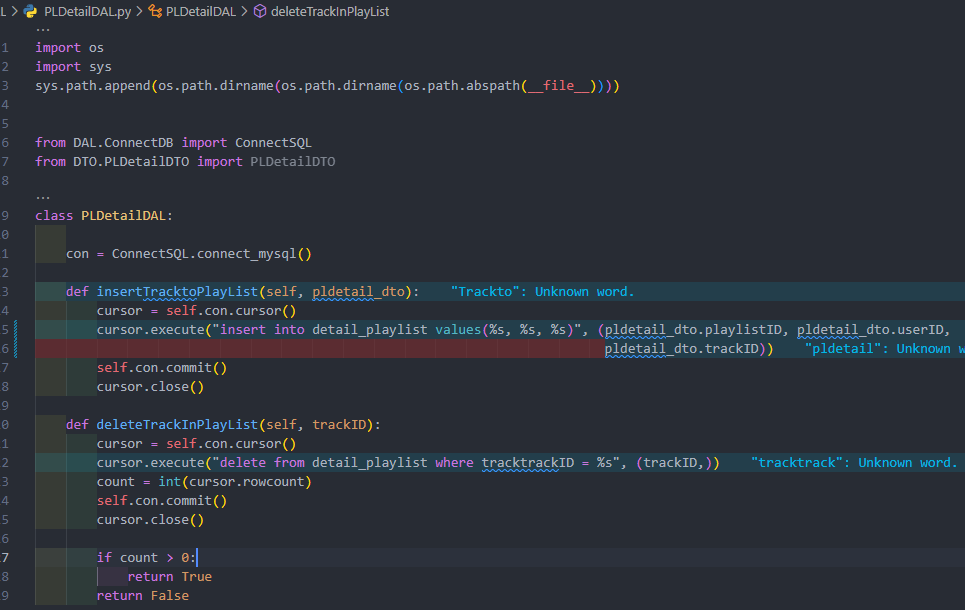
\includegraphics[width=\textwidth]{images/PlayListDetail.png}
	\caption{Code cho class PLDetailDAL gồm 2 phương thức thêm và xóa}
\end{figure}
\begin{flushleft}
	-Giải thích:
	\begin{itemize}
		\item Phương thức \textbf{insertTracktoPlayList(self, pldetail\_dto)} thêm một bài hát vào playlist.

		\item Phương thức \textbf{deleteTrackInPlayList(playlistID, trackID)} xóa một bài hát khỏi playlist theo trackID.

	\end{itemize}
\end{flushleft}

\clearpage
\newpage
\begin{figure}[h]
	\centering
	\includegraphics[width=\textwidth]{images/TrackDAL.png}
	\caption{Code cho class TrackDAL gồm các phương thức CRUD (Create, Read, Update, Delete)}
\end{figure}
\clearpage
\newpage
\begin{flushleft}
	-Giải thích:
	\begin{itemize}
		\item Phương thức \textbf{getAllData(self)} trả về danh sách tất cả các bài hát trong cơ sở dữ liệu.

		\item Phương thức \textbf{generateTrackID(self)} tạo một ID duy nhất cho bài hát mới.
		      \begin{flushleft}
			      +Chi tiết hơn:

			      -Đầu tiên, ta sẽ thiết lập kết nối đến cơ sở dữ liệu.

			      -Sau đó, ta sẽ tạo 1 cursor từ kết nối này để thực hiện các thao tác truy vấn dữ liệu.

			      -Ta thực hiện câu lệnh SQL để lấy ID cao nhất (mới nhất) từ bảng track.

			      -Chúng ta lấy kết quả ở dòng đầu tiên của câu lệnh truy vấn. Nếu kết quả tồn tại (tức là bảng không trống), ta lấy ID này, loại bỏ ký tự đầu tiên (giả sử là 'T'), chuyển phần còn lại thành số và cộng thêm một để tạo ID mới.

			      -Nếu kết quả không tồn tại (tức là bảng trống), ta sẽ bắt đầu với ID là 1.

			      -Cuối cùng, ta trả về ID mới này dưới dạng chuỗi, thêm tiền tố 'T' và đảm bảo rằng nó có độ dài 4 ký tự bằng cách thêm các số 0 vào đầu.
		      \end{flushleft}

		\item Phương thức \textbf{insert(self, track\_dto)} thêm một bài hát mới vào cơ sở dữ liệu.

		\item Phương thức \textbf{update(track\_dto)} sửa thông tin của một bài hát.

		\item Phương thức \textbf{deleteTrack(trackID)} xóa một bài hát dựa vào id.

	\end{itemize}
\end{flushleft}
\clearpage

\newpage
\begin{figure}[h]
	\centering
	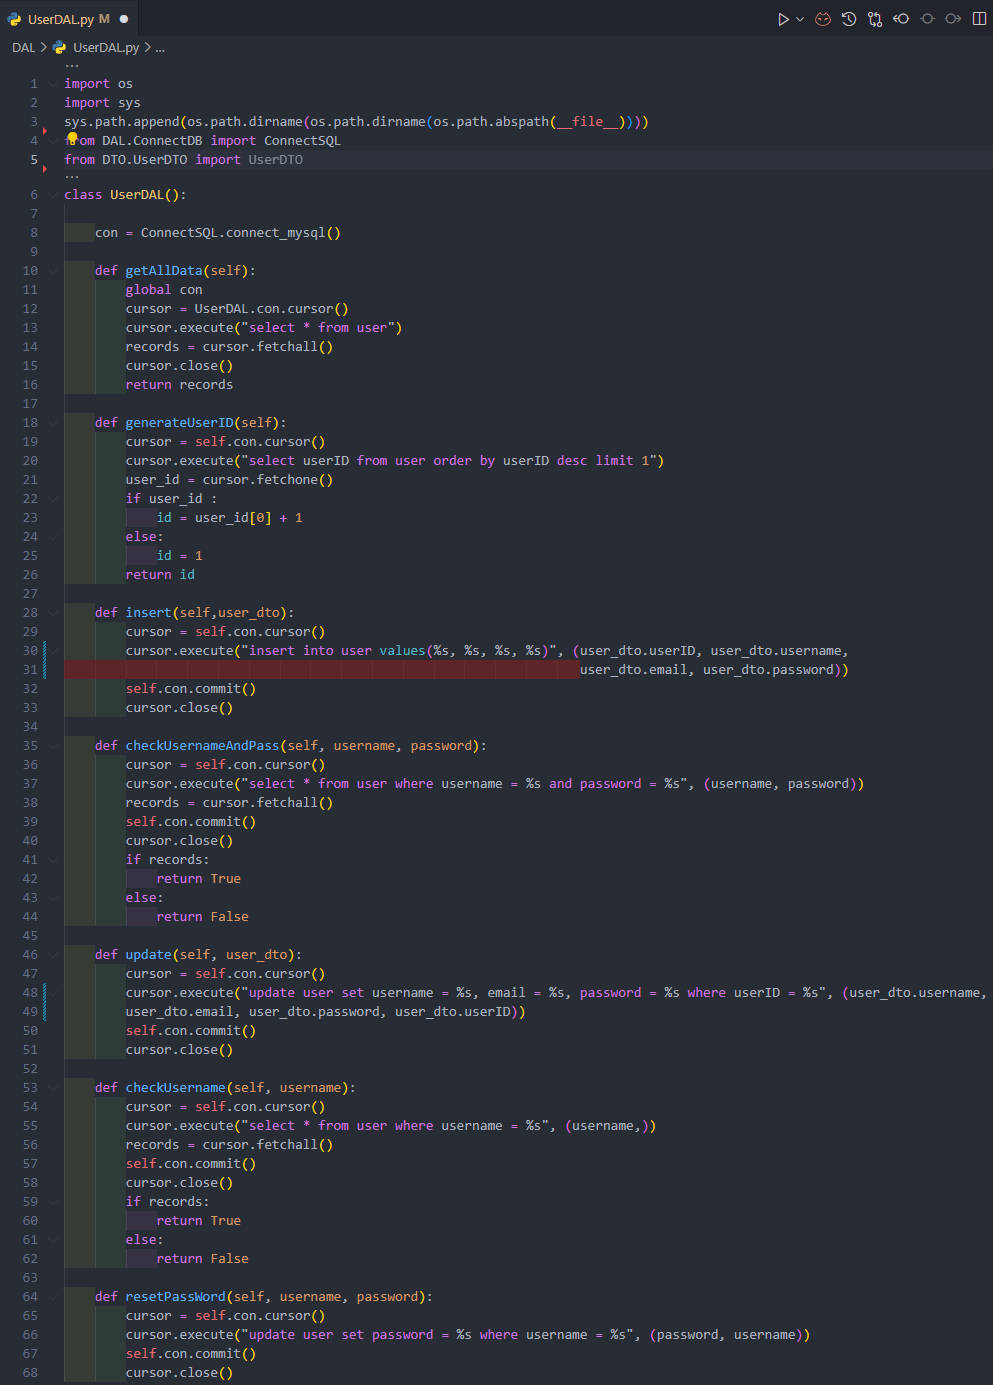
\includegraphics[width=\textwidth]{images/userDAL.png}
	\caption{Code cho class UserDAL gồm các phương thức CRUD (Create, Read, Update, Delete)}
\end{figure}
\clearpage
\newpage
\begin{flushleft}
	-Giải thích:
	\begin{itemize}
		\item Phương thức \textbf{getAllData(self)} trả về danh sách tất cả các user trong cơ sở dữ liệu.

		\item Phương thức \textbf{generateUserID(self)} tạo một ID duy nhất cho user mới.

		\item Phương thức \textbf{checkUsernameAndPass(self, user\_dto)} kiểm tra username và password của user.

		\item Phương thức \textbf{insert(self, user\_dto)} thêm một user mới vào cơ sở dữ liệu.

		\item Phương thức \textbf{update(self, user\_dto)} sửa thông tin của một user.

		\item Phương thức \textbf{checkUsername(self, userID)} kiểm tra username của user.

		\item Phương thức \textbf{resetPassword(self, username, password)} reset password của user.

	\end{itemize}
	-Sau khi hoàn thành các class ở tầng DAL, chúng ta sẽ tiến hành tạo các class ở tầng BLL (Business Logic Layer) để thực hiện các thao tác xử lý logic cho ứng dụng.
	\begin{figure}[h]
		\centering
		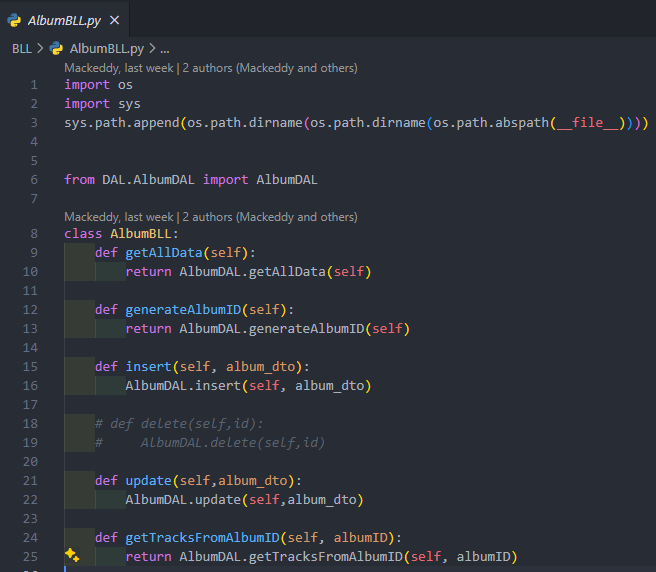
\includegraphics[width=0.9\textwidth]{images/AlbumBLL.png}
		\caption{Code cho class AlbumBLL gồm các phương thức xử lý logic}
	\end{figure}

\end{flushleft}
\clearpage
\newpage
\begin{figure}[h]
	\centering
	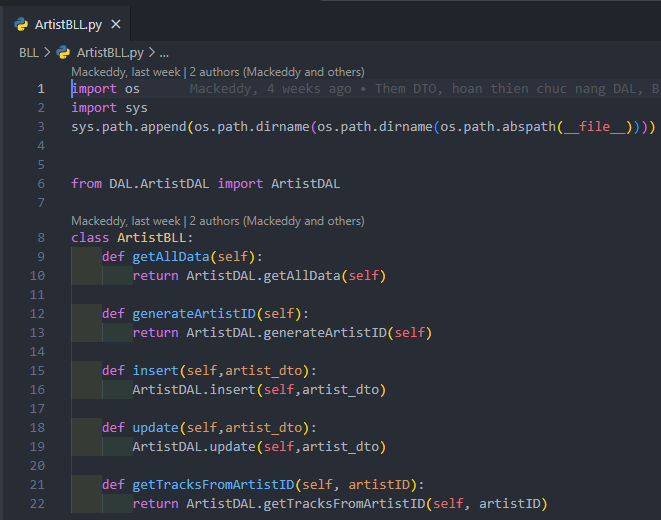
\includegraphics[width=0.8\textwidth]{images/artistBLL.png}
	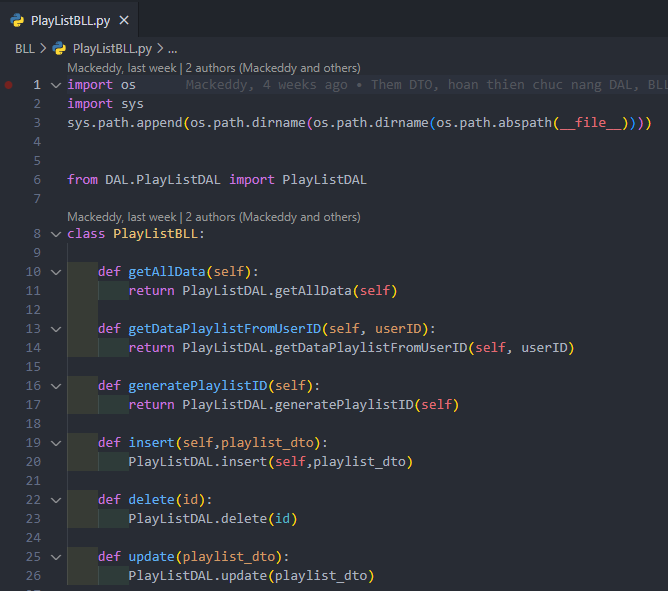
\includegraphics[width=0.8\textwidth]{images/PlayListBLL.png}
	\caption{Code cho class ArtistBLL, PlayListBLL gồm các phương thức xử lý logic}
\end{figure}

\clearpage
\newpage
\begin{figure}[h]
	\centering
	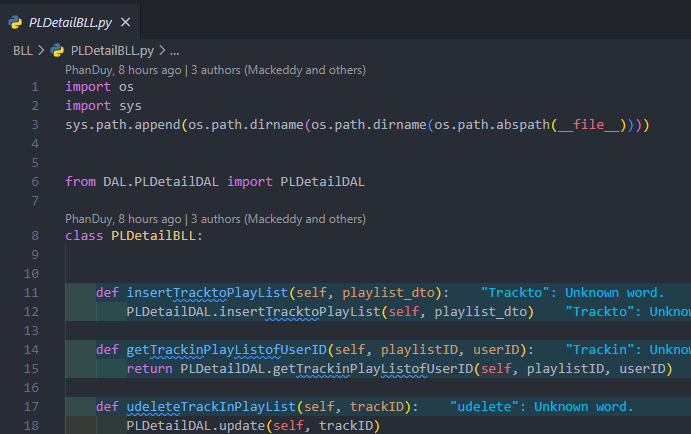
\includegraphics[width=0.8\textwidth]{images/PlayListDetailBLL.png}
	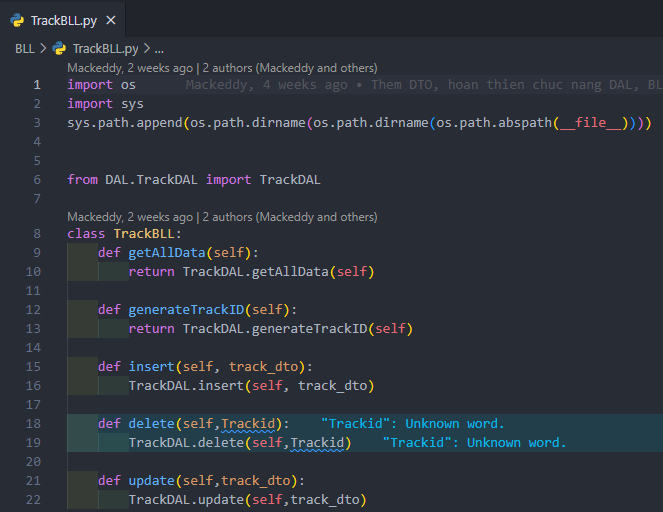
\includegraphics[width=0.8\textwidth]{images/TrackBLL.png}
	\caption{Code cho class PLDetailBLL, TrackBLL gồm các phương thức xử lý logic}
\end{figure}
\clearpage
\newpage
\begin{figure}[h]
	\centering
	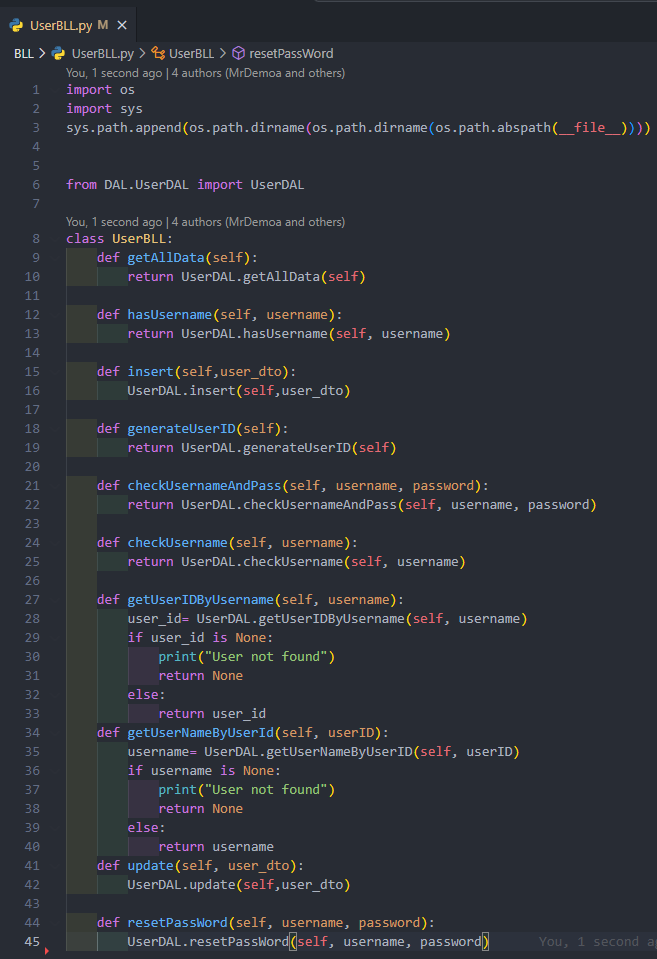
\includegraphics[width=0.8\textwidth]{images/UserBLL.png}
	\caption{Code cho class UserBLL gồm các phương thức xử lý logic}
\end{figure}
\clearpage
\newpage
\begin{flushleft}
	-Sau khi hoàn thành việc thiết lập các phương thức xử lý tại các tầng BLL và DAL,
	chúng ta sẽ tiếp tục tạo các lớp (class) tại tầng GUI (Graphical User Interface). Mục đích của việc này là để thực hiện các thao tác giao diện cho ứng dụng.

	-Đồng thời, chúng ta sẽ sử dụng thư viện Tkinter để tạo giao diện cho ứng dụng.

	-Thư viện PIL (Python Imaging Library) sẽ được sử dụng để hiển thị hình ảnh trong ứng dụng.

	-Thư viện Pygame.mixer sẽ được sử dụng để phát nhạc trong ứng dụng.

	-Thư viện mutagen sẽ được sử dụng để lấy thông tin về file nhạc như tên bài hát, tên nghệ sĩ, và album.

	-Ngoài ra, chúng ta cũng sẽ sử dụng thư viện socket để tạo kết nối giữa client và server.
	Điều này giúp cho việc truyền dữ liệu giữa client và server trở nên dễ dàng hơn.

	\subsubsection{Thiết kế socket server và client và cài đặt vài chức năng cho ứng dụng nghe nhạc}
	\begin{flushleft}
		-Để tạo kết nối giữa client và server, chúng ta sẽ tạo một socket server và một socket client.

		-Server sẽ lắng nghe các yêu cầu từ client và thực hiện các thao tác tương ứng.

		-Client sẽ gửi các yêu cầu đến server và nhận kết quả trả về từ server.

		-Chúng ta sẽ tuân theo mô hình client-server để tạo kết nối giữa client và server như sau:
		\begin{figure}[h]
			\centering
			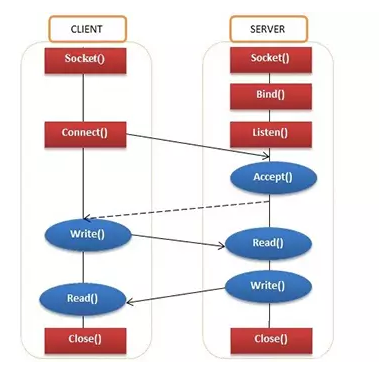
\includegraphics[width=0.6\textwidth]{images/socket-establishment.png}
			\caption{Thiết kế socket server và client cho ứng dụng nghe nhạc}
		\end{figure}

		-Trước tiên, chúng ta sẽ mở một cổng kết nối trên server và lắng nghe các yêu cầu từ client.
	\end{flushleft}
\end{flushleft}
\clearpage
\newpage
\begin{flushleft}
	\begin{figure}[h]
		\centering
		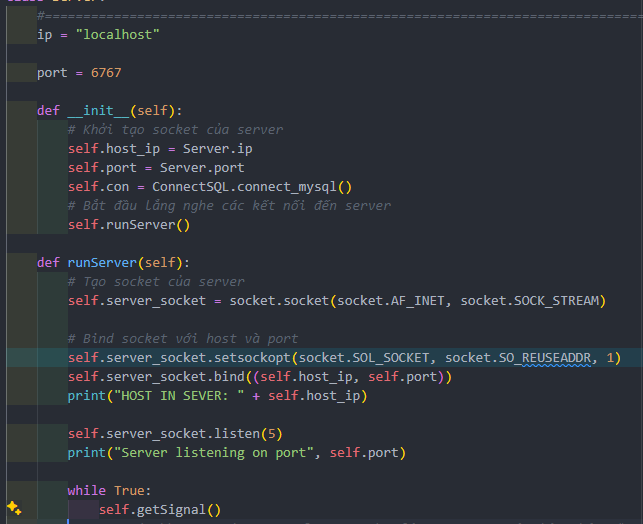
\includegraphics[width=0.6\textwidth]{images/Server-establishment.png}
		\caption{Code server gồm phương thức khởi tạo và chạy server}
	\end{figure}
	+Giải thích:

	-Phương thức \textbf{init(self)} khởi tạo server, gán ip và port, thiết lập kết nối đến cơ sở dữ liệu thông qua class ConnectDB.

	-Phương thức \textbf{run(self)} chạy server, lắng nghe các yêu cầu từ client và thực hiện các thao tác tương ứng.
\end{flushleft}
\clearpage
\newpage
\begin{figure}
	\centering
	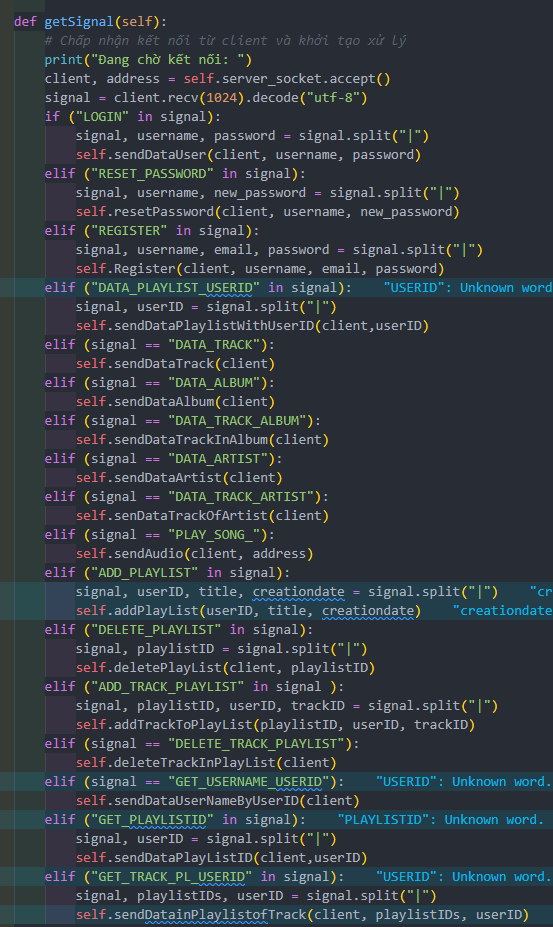
\includegraphics[width=0.7\textwidth]{images/getSignal-server.png}
	\caption{Code server-side phương thức lấy phản hồi từ client}
\end{figure}
\clearpage
\newpage
\begin{flushleft}
	-Ví dụ:

	+Ở chức năng đăng nhập tài khoản, khi client gửi yêu cầu đến server, server sẽ kiểm tra thông tin đăng nhập của user và trả về kết quả cho client.

	+Server sẽ gọi xuống cơ sở dữ liệu để kiểm tra thông tin đăng nhập của user và trả về kết quả cho server.

	+Server sẽ trả về kết quả cho client và client sẽ hiển thị thông báo tương ứng với kết quả đó.
	+Tương tự như vậy với các hàm khác như Reset Password, Register, Send PlayList, Send Track, Send Album, Send Artist, \dots
	\begin{figure}
		\centering
		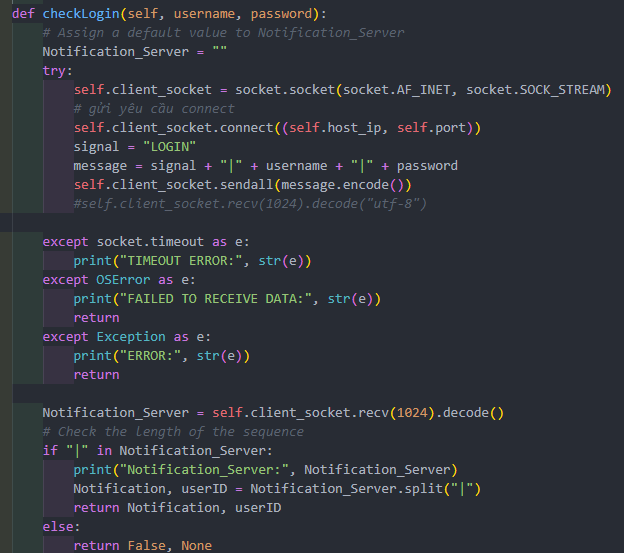
\includegraphics[width=0.7\textwidth]{images/checkLogin-Client.png}
		\caption{Code cho client-side phương thức kiểm tra thông tin đăng nhập của user ở client-side}
	\end{figure}
	\begin{figure}
		\centering
		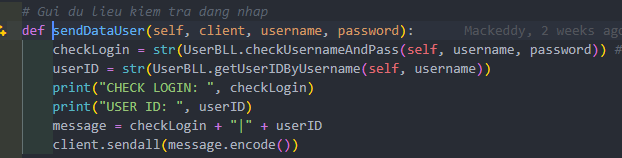
\includegraphics[width=0.7\textwidth]{images/sendDataUser-Server.png}
		\caption{Code cho server-side phương thức kiểm tra thông tin đăng nhập của user ở server-side}
	\end{figure}
\end{flushleft}
\clearpage
\newpage
\begin{flushleft}
	\begin{figure}
		\centering
		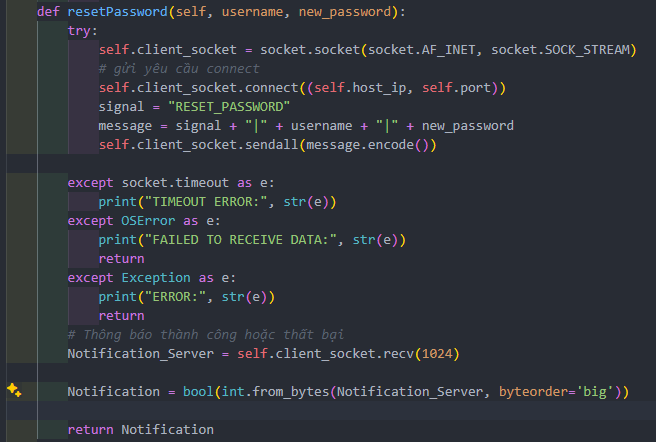
\includegraphics[width=0.5\textwidth]{images/resetPassword-client.png}
		\caption{Code cho client-side xử lý đặt lại mật khẩu của user và gửi yêu cầu đến server-side}
	\end{figure}

	\begin{figure}
		\centering
		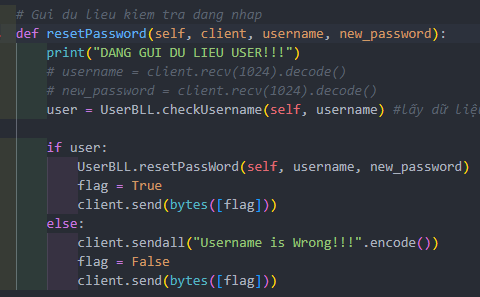
\includegraphics[width=0.5\textwidth]{images/resetPassword-server.png}
		\caption{Code cho server-side đặt lại mật khẩu của user và trả về kết quả cho client-side}
	\end{figure}

	-Giải thích:

	Hàm resetPassword cho client:

	+Đầu tiên, hàm tạo một socket mới và kết nối đến server thông qua IP và cổng đã cho.

	+Sau đó, hàm tạo một chuỗi tin nhắn bằng cách nối chuỗi ``RESET\_PASSWORD'' với tên người dùng và mật khẩu mới, rồi gửi tin nhắn này đến Server.

	+Nếu có lỗi xảy ra trong quá trình này (như timeout hoặc lỗi hệ thống), hàm sẽ in ra thông báo lỗi và trả về.

	+Cuối cùng, hàm nhận thông báo từ server, chuyển đổi nó thành boolean và trả về. Thông báo này cho biết việc đặt lại mật khẩu có thành công hay không.

	Hàm resetPassword cho server:

	+Đầu tiên, hàm in ra thông báo “DANG GUI DU LIEU USER!!!” để cho biết rằng nó đang xử lý dữ liệu người dùng.

	+Sau đó, hàm kiểm tra xem tên người dùng có tồn tại trong cơ sở dữ liệu hay không bằng cách gọi hàm UserBLL.checkUsername.

	+Nếu tên người dùng tồn tại, hàm sẽ đặt lại mật khẩu bằng cách gọi hàm UserBLL.resetPassWord, gán cờ thành True và gửi cờ này đến client.

	+Nếu tên người dùng không tồn tại, hàm sẽ gửi thông báo “Username is Wrong!!!” đến client và gán biến False.
\end{flushleft}
\clearpage
\newpage
\begin{flushleft}
	\begin{figure}
		\centering
		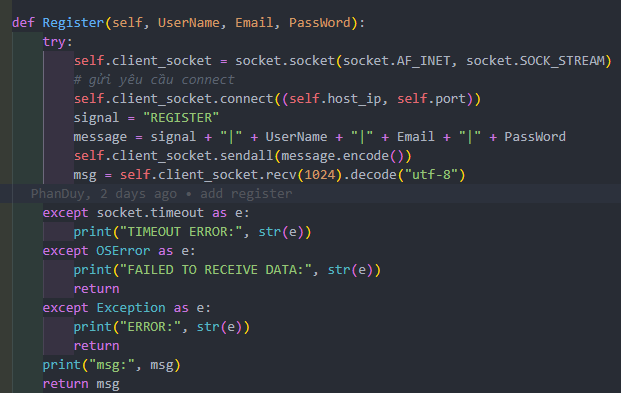
\includegraphics[width=0.6\textwidth]{images/register-client.png}
		\caption{Code cho client-side xử lý đăng ký tài khoản và gửi yêu cầu đến server-side}
	\end{figure}
	\begin{figure}
		\centering
		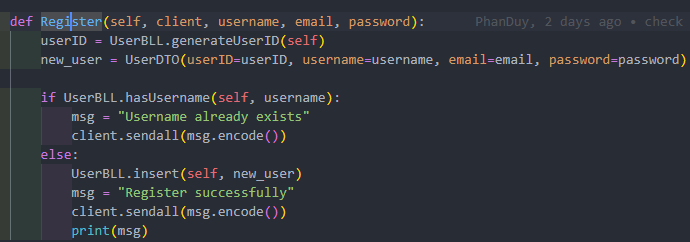
\includegraphics[width=0.6\textwidth]{images/register-server.png}
		\caption{Code cho server-side xử lý đăng ký tài khoản và trả về kết quả cho client-side}
	\end{figure}

	-Giải thích:

	-Hàm Register cho client:

	+Đầu tiên, hàm tạo một socket mới và kết nối đến server thông qua IP và cổng đã cho.

	+Sau đó, hàm tạo một chuỗi tin nhắn bằng cách nối chuỗi “REGISTER” với tên người dùng, email và mật khẩu, rồi gửi tin nhắn này đến server.

	+Nếu có lỗi xảy ra trong quá trình này (như timeout hoặc lỗi hệ thống), hàm sẽ in ra thông báo lỗi và trả về.

	+Cuối cùng, hàm nhận thông báo từ server và trả về. Thông báo này cho biết việc đăng ký có thành công hay không.

	-Hàm Register cho server:

	+Đầu tiên, hàm tạo một ID người dùng mới bằng cách gọi hàm UserBLL.generateUserID\@.

	+Sau đó, hàm tạo một đối tượng người dùng mới với ID người dùng, tên người dùng, email và mật khẩu.

	+Hàm kiểm tra xem tên người dùng đã tồn tại trong cơ sở dữ liệu hay chưa bằng cách gọi hàm UserBLL.hasUsername.

	+Nếu tên người dùng đã tồn tại, hàm sẽ gửi thông báo “Username already exists” đến client.

	+Nếu người dùng chưa tồn tại, hàm sẽ thêm người dùng mới vào cơ sở dữ liệu qua gọi hàm UserBLL.insert, gửi thông báo “Register successfully” đến client và in thông báo này ra màn hình.
\end{flushleft}
\clearpage
\newpage
\begin{flushleft}
	\begin{figure}
		\centering
		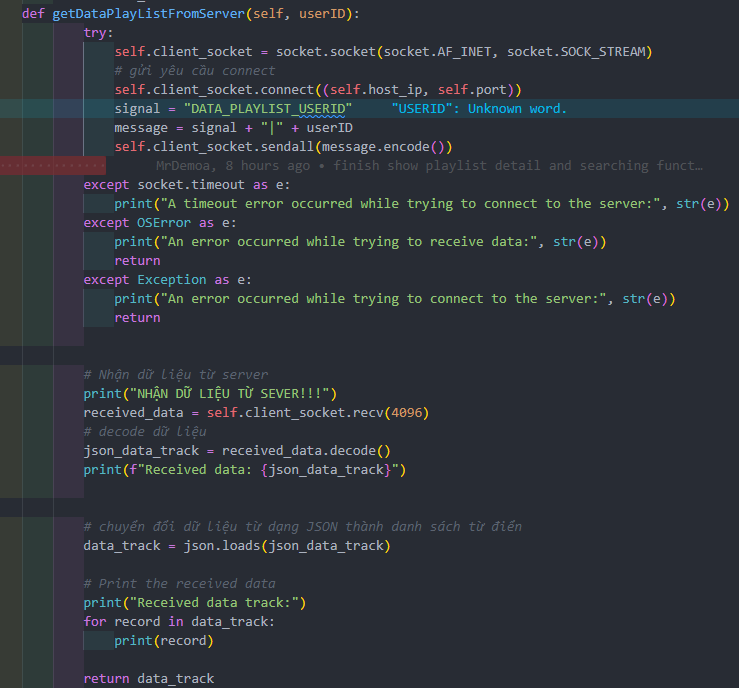
\includegraphics[width=0.5\textwidth]{images/getDataPlayListFromServer-Client.png}
		\caption{Code cho client-side lấy danh sách playlist đến client-side qua user-id}
	\end{figure}
	\begin{figure}
		\centering
		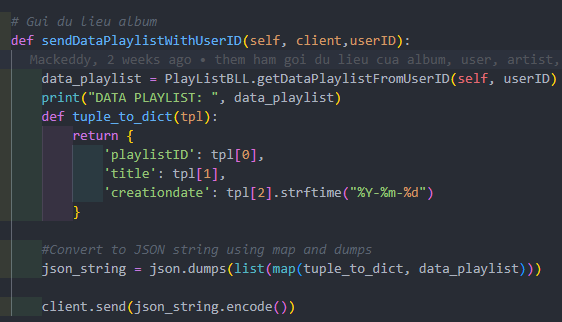
\includegraphics[width=0.6\textwidth]{images/sendDataPlayListWithUserId-Server.png}
		\caption{Code cho server-side gửi dữ liệu playlist đến client-side qua user-id}
	\end{figure}

	-Hàm getDataPlayListFromServer cho client:

	+Đầu tiên, hàm tạo một socket mới và kết nối đến server thông qua IP và cổng đã cho.

	+Sau đó, hàm tạo một chuỗi tin nhắn bằng cách nối chuỗi ``DATA\_PLAYLIST\_USERID'' với userID, rồi gửi tin nhắn này đến server.

	+Nếu có lỗi xảy ra trong quá trình này (như timeout hoặc lỗi hệ thống), hàm sẽ in ra thông báo lỗi và trả về.

	+Cuối cùng, hàm nhận dữ liệu từ server, giải mã dữ liệu này từ dạng JSON thành danh sách từ điển, và trả về danh sách này.

	-Hàm sendDataPlaylistWithUserID cho server:

	+Đầu tiên, hàm lấy dữ liệu playlist từ cơ sở dữ liệu bằng cách gọi hàm PlayListBLL.getDataPlaylistFromUserID\@.

	+Sau đó, hàm chuyển đổi dữ liệu này từ dạng tuple thành từ điển\@, rồi chuyển đổi từ điển này thành chuỗi JSON\@.

	+Cuối cùng, hàm gửi chuỗi JSON này đến client.
\end{flushleft}
\clearpage
\newpage
\subsubsection{Xây dựng giao diện và chức năng cho ứng dụng}
\subsubsubsection{Đăng nhập}
-Sau khi chúng ta đã hoàn thành thiết lập các chức năng cần thiết cho Server và Client để tạo kết nối giữa chúng,
chúng ta sẽ tiến hành tạo giao diện cho ứng dụng và kết hợp các chức năng đã thiết lập ở trên vào giao diện.

-Đầu tiên, chúng ta có giao diện đăng nhập cho ứng dụng:

\begin{figure}[h]
	\centering
	\includegraphics[width=0.6\textwidth]{images/login.png}
	\caption{Giao diện đăng nhập cho ứng dụng}
\end{figure}

-Ở đây chúng ta có 2 ô nhập liệu là username và password, và 3 nút chức năng là Login, Register và Reset Password.

\clearpage
\newpage
\begin{flushleft}
	\subsubsubsection{Đăng kí}
	- Khi chúng ta bấm Sign Up, chúng ta sẽ chuyển sang giao diện đăng ký tài khoản như phía dưới:
	\begin{figure}[h]
		\centering
		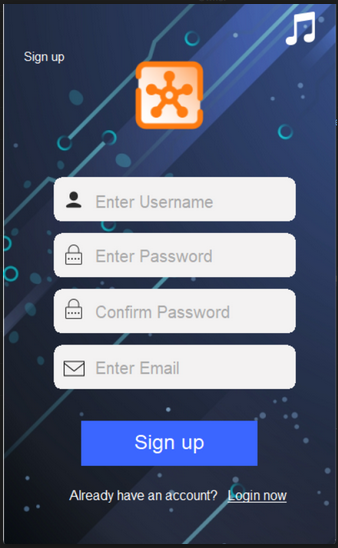
\includegraphics[width=0.4\textwidth]{images/signup.png}
		\caption{Giao diện đăng ký tài khoản cho ứng dụng}
	\end{figure}

	\subsubsubsection{Đặt lại mật khẩu}
	- Khi chúng ta bấm Reset Password, chúng ta sẽ chuyển sang giao diện đặt lại mật khẩu như phía dưới:
	\begin{figure}[h]
		\centering
		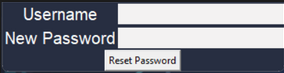
\includegraphics[width=0.6\textwidth]{images/resetPassword.png}
		\caption{Giao diện đặt lại mật khẩu cho ứng dụng}
	\end{figure}
\end{flushleft}
\clearpage
\newpage
\begin{flushleft}
	\subsubsection{Trang chủ}
	- Sau khi đăng nhập thành công, chúng ta sẽ chuyển sang giao diện chính của ứng dụng như phía dưới:
	\begin{figure}[h]
		\centering
		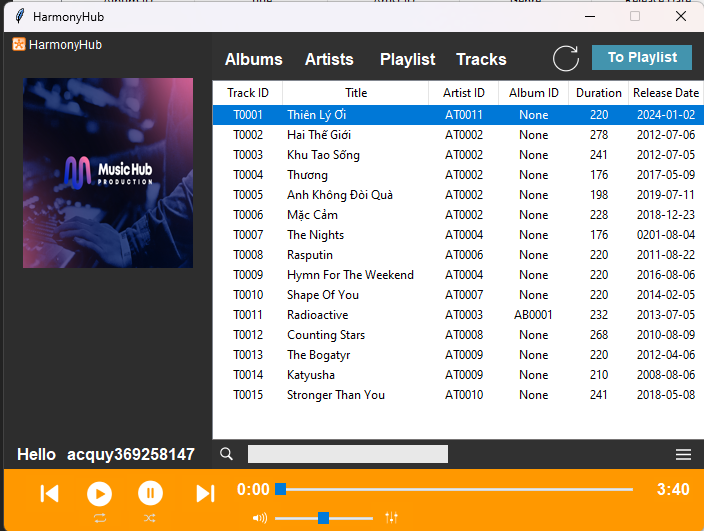
\includegraphics[width=0.8\textwidth]{images/MainUI-User.png}
		\caption{Giao diện chính của ứng dụng sau khi đăng nhập thành công}
	\end{figure}

	-Ở đây chúng ta có 4 tab chính là Playlist, Albums, Artists và Tracks và nhiều nút chức năng khác như Play, Pause, Next, Previous, Volume, thêm bài hát vào Playlist \dots

	\subsubsection{Tìm kiếm}
	-Tìm kiếm ở đây là tìm kiếm theo tên bài hát, chúng ta chỉ cần nhập tên bài hát vào ô tìm kiếm và bấm nút Search để tìm kiếm.
	\begin{figure}[h]
		\centering
		
\includegraphics[width=0.8\textwidth]{images/search.png}
		\caption{Giao diện tìm kiếm bài hát theo tên}
	\end{figure}
\end{flushleft}
\clearpage
\newpage
\begin{figure}
	\centering
	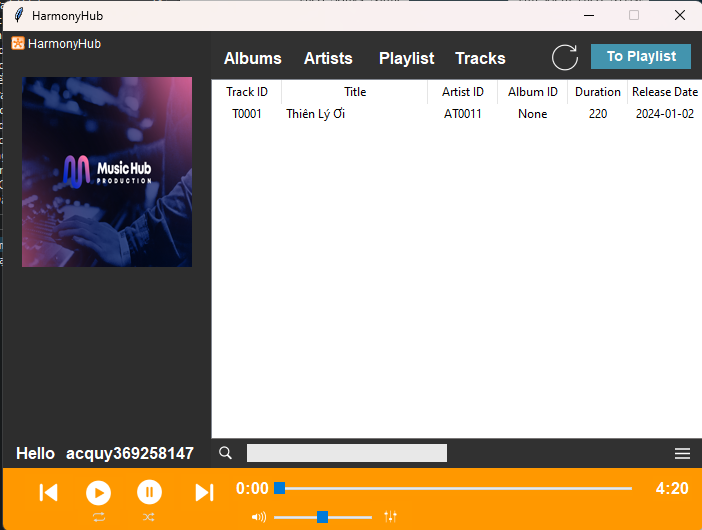
\includegraphics[width=0.8\textwidth]{images/UIaftersearching.png}
	\caption{Kết quả tìm kiếm bài hát theo tên}
\end{figure}
\subsubsection{Nghe nhạc}
\begin{flushleft}
	- Để nghe nhạc, chúng ta chỉ cần chọn bài hát từ danh sách bài hát và bấm nút Play.

	- Giao diện bài hát đang phát gồm các chức năng như Play
\includegraphics[width=0.5cm]{images/play-icon.png}, Pause
\includegraphics[width=0.5cm]{images/pause-icon.png}, Next
\includegraphics[width=0.5cm]{images/nextsong-icon.png}, Previous
\includegraphics[width=0.5cm]{images/prevsong-icon.png}, Volume\includegraphics[width=1cm]{images/volume-bar.png}, thêm bài hát vào Playlist \dots

	- Giao diện chính để thao tác với bài hát đang phát:

	- Để dừng nghe nhạc, chúng ta chỉ cần bấm nút tạm ngừng \includegraphics[width=0.5cm]{images/pause-icon.png}.
	\begin{figure}[h]
		\centering
		\includegraphics[width=0.8\textwidth]{images/mainUicontrolMusic.png}
		\caption{Giao diện chính mỗi bài nhạc}
	\end{figure}
	\subsubsection{Playlist}
	-Ngoài các thao tác với mỗi bài nhạc, chúng ta có thể thêm bài hát vào Playlist bằng cách chọn bài hát và bấm vào nút playlist\includegraphics[width=1cm]{images/addplaylist-button.png}.

	-Sau khi bấm vào, nó sẽ hiện cửa sổ chọn Playlist để thêm bài hát vào Playlist đó.
\end{flushleft}
\clearpage
\newpage
\begin{flushleft}
	\begin{figure}[h]
		\centering
		\includegraphics[width=0.4\textwidth]{images/newplaylist.png}
		\caption{Giao diện thêm bài hát vào Playlist}
	\end{figure}

	-Sau khi chọn Playlist, bài hát được chọn sẽ được thêm vào Playlist đó.
	\begin{figure}[h]
		\centering
		\includegraphics[width=0.8\textwidth]{images/playlistdetailUI.png}
		\caption{Giao diện Playlist}
	\end{figure}

	-Ta nhấn đúp vào playlist để xem danh sách bài hát trong playlist đó.
\end{flushleft}
\clearpage
\newpage
\begin{flushleft}
	\begin{figure}[h]
		\centering
		\includegraphics[width=0.8\textwidth]{images/showsongsinplaylist.png}
		\caption{Danh sách bài hát trong Playlist}
	\end{figure}
	\subsubsection{Giao diện và chức năng cho Server}
	\subsubsubsection{Quản lý nhạc}
	-Hiển thị danh sách bài hát:
\end{flushleft}
\clearpage
\newpage
\begin{flushleft}
	\begin{figure}[h]
		\centering
		\includegraphics[width=0.9\textwidth]{images/admin-mainUI.png}
		\caption{Danh sách bài hát}
	\end{figure}
	-Danh sách bài hát trong kho lưu trữ gồm id, tên bài hát, mã nghệ sĩ, mã album, thời lượng, và ngày phát hành.
	\subsubsubsection{Thêm bài hát mới}
	-Sau khi điền đẩy đủ các thông tin, chúng ta bấm nút Add để thêm bài hát mới vào kho lưu trữ.
	\begin{figure}[h]
		\centering
		\includegraphics[width=0.3\textwidth]{images/addnewsong.png}
		\caption{Thêm bài hát mới}
	\end{figure}
\end{flushleft}
\clearpage
\newpage
\begin{flushleft}
	\begin{figure}
		\centering
		\includegraphics[width=0.9\textwidth]{images/shownewsongadded.png}
		\caption{Thêm bài hát mới thành công}
	\end{figure}
	-Sau khi thêm bài hát mới thành công, nó sẽ hiện ra trong danh sách bài hát và chúng ta kéo thả file nhạc vào thư mục SongList của Resource để thêm bài hát mới vào kho lưu trữ.

	-Đổi tên thư mục ứng với ID của bài hát mới.
	\begin{figure}[h]
		\centering
		\includegraphics[width=0.2\textwidth]{images/song-resources.png}
		\caption{Thêm bài hát mới vào thư mục SongList}
	\end{figure}
	\subsubsubsection{Chỉnh sửa bài hát}
	-Để chỉnh sửa bài hát, chúng ta chọn bài hát cần chỉnh sửa và bấm nút Edit\includegraphics[width=1cm]{images/editbutton.png}. Sau khi chỉnh
	các thông tin cần thiết, chúng ta bấm nút Save để lưu lại.
\end{flushleft}
\clearpage
\newpage
\begin{flushleft}
	\begin{figure}
		\centering
		\includegraphics[width=0.4\textwidth]{images/editform.png}
		\caption{Giao diện chỉnh sửa bài hát}
	\end{figure}
	\begin{figure}[h]
		\centering
		\includegraphics[width=0.8\textwidth]{images/beforeediting.png}
		\caption{Thông tin bài hát trước khi chỉnh sửa}
	\end{figure}
	-Sau khi chỉnh sửa bài hát, nó sẽ hiện ra thông báo chỉnh sửa thành công.
\end{flushleft}
\clearpage
\newpage
\begin{flushleft}
	\begin{figure}[h]
		\centering
		\includegraphics[width=0.8\textwidth]{images/afterediting.png}
		\caption{Thông tin bài hát sau khi chỉnh sửa}
	\end{figure}
	\subsubsubsection{Xóa bài hát}
	-Để xóa bài hát, chúng ta chọn bài hát cần xóa và bấm nút Delete\includegraphics[width=1cm]{images/deletebutton.png}.
	\begin{figure}[h]
		\centering
		\includegraphics[width=0.8\textwidth]{images/afterdeleting.png}
		\caption{Bài hát được chọn sau khi xóa (mã T0016)}
	\end{figure}
	\subsubsection{Quản lý danh sách Album}
	-Hiển thị danh sách các Album trong cơ sở dữ liệu.
\end{flushleft}
\clearpage
\newpage
\begin{flushleft}
	\begin{figure}
		\centering
		\includegraphics[width=0.8\textwidth]{images/albumlist.png}
		\caption{Danh sách Album}
	\end{figure}
	-Danh sách được hiển thị gồm mã album, tên album, mã nghệ sĩ, thể loại và ngày phát hành.
	\subsubsubsection{Thêm Album mới}
	-Chúng ta bấm vào nút Add Albums\includegraphics[width=1cm]{images/addalbumsbutton.png} sau đó hệ thống sẽ hiện ra giao diện thêm Album mới.
	\begin{figure}[h]
		\centering
		\includegraphics[width=0.4\textwidth]{images/addnewalbumform.png}
		\caption{Thêm Album mới}
	\end{figure}

	-Chúng ta điền toàn bộ thông tin cần thiết sau đó bấm Submit để thêm Album mới vào cơ sở dữ liệu.
\end{flushleft}
\clearpage
\newpage
\begin{flushleft}
	\begin{figure}
		\centering
		\includegraphics[width=0.8\textwidth]{images/afteraddingnewalbum.png}
		\caption{Giao diện sau khi thêm Album mới thành công}
	\end{figure}
	\subsubsubsection{Chỉnh sửa Album}
	-Để chỉnh sửa Album, chúng ta chọn Album cần chỉnh sửa và bấm nút Edit\includegraphics[width=1cm]{images/editAlbumbutton.png}.
	\begin{figure}[h]
		\centering
		\includegraphics[width=0.8\textwidth]{images/editalbumform.png}
		\caption{Giao diện chỉnh sửa Album}
	\end{figure}

	-Sau khi chỉnh sửa xong các thông tin cần thay đổi, chúng ta bấm nút Save để lưu lại.
	\begin{figure}[h]
		\centering
		\includegraphics[width=0.8\textwidth]{images/aftereditalbum.png}
		\caption{Giao diện sau khi chỉnh sửa Album}
	\end{figure}
\end{flushleft}
\clearpage
\newpage
\begin{flushleft}
	\subsubsection{Quản lý thông tin nghệ sĩ}
	\subsubsubsection{Hiển thị danh sách nghệ sĩ}
	-Chúng ta bấm vào mục Artist để hiển thị danh sách nghệ sĩ.
	\begin{figure}[h]
		\centering
		\includegraphics[width=0.8\textwidth]{images/formartists.png}
		\caption{Danh sách các nghệ sĩ}
	\end{figure}

	-Danh sách nghệ sĩ gồm mã nghệ sĩ, tên nghệ sĩ, và thể loại nhạc mà nghệ sĩ đó thể hiện.

	\subsubsubsection{Thêm nghệ sĩ mới}
	-Chúng ta bấm vào nút Add Artists\includegraphics[width=1cm]{images/addartists.png} để thêm nghệ sĩ mới.

	-Sau đó, hệ thống sẽ hiển thị giao diện thêm nghệ sĩ mới.

	\begin{figure}[h]
		\centering
		\includegraphics[width=0.3\textwidth]{images/addartistform.png}
		\caption{Thêm nghệ sĩ mới}
	\end{figure}
	-Ta điền các thông tin cần thiết sau đó bấm Submit để thêm nghệ sĩ mới vào cơ sở dữ liệu.
\end{flushleft}
\clearpage
\newpage
\begin{flushleft}
	\begin{figure}
		\centering
		\includegraphics[width=0.8\textwidth]{images/newartistafteradding.png}
		\caption{Giao diện sau khi thêm nghệ sĩ mới thành công}
	\end{figure}
	\subsubsubsection{Chỉnh sửa thông tin nghệ sĩ}
	-Để chỉnh sửa thông tin nghệ sĩ, chúng ta chọn nghệ sĩ cần chỉnh sửa và bấm nút Edit\includegraphics[width=1cm]{images/editbutton.png}.

	\begin{figure}
		\centering
		\includegraphics[width=0.8\textwidth]{images/editartistform.png}
		\caption{Giao diện chỉnh sửa thông tin nghệ sĩ trước khi chỉnh sửa}
	\end{figure}

	\begin{figure}
		\centering
		\includegraphics[width=0.8\textwidth]{images/aftereditingartist.png}
		\caption{Giao diện chỉnh sửa thông tin nghệ sĩ sau khi chỉnh sửa}
	\end{figure}

	-Sau khi chỉnh sửa xong, ta thấy tên nghệ sĩ đã được thay đổi.
\end{flushleft}
\clearpage
\newpage
\begin{flushleft}

	\subsubsection{Quản lý người dùng}
	\subsubsubsection{Hiển thị danh sách người dùng}
	-Chúng ta bấm vào mục User để hiển thị danh sách người dùng.
	\begin{figure}[h]
		\centering
		\includegraphics[width=0.8\textwidth]{images/formusers.png}
		\caption{Danh sách người dùng}
	\end{figure}

	-Danh sách người dùng gồm mã người dùng, tên người dùng, email, và mật khẩu.

	\subsubsubsection{Thêm người dùng mới}
	-Chúng ta bấm vào nút Add Users\includegraphics[width=1cm]{images/adduserbtn.png} để thêm người dùng mới.

	-Sau đó, hệ thống sẽ hiển thị giao diện thêm người dùng mới.
	\begin{figure}[h]
		\centering
		\includegraphics[width=0.3\textwidth]{images/addnewuser.png}
		\caption{Thêm người dùng mới}
	\end{figure}
\end{flushleft}
\clearpage
\newpage
\begin{flushleft}
	-Ta điền các thông tin cần thiết sau đó bấm Submit để thêm người dùng mới vào cơ sở dữ liệu.
	\begin{figure}[h]
		\centering
		\includegraphics[width=0.8\textwidth]{images/afteraddingnewuser.png}
		\caption{Giao diện sau khi thêm người dùng mới thành công}
	\end{figure}

	-Sau khi thêm người dùng mới thành công, hệ thống sẽ hiển thị thông báo thêm người dùng mới thành công và hiển thị người dùng mới trong danh sách người dùng.
	\subsubsubsection{Chỉnh sửa thông tin người dùng}
	-Để chỉnh sửa thông tin người dùng, chúng ta chọn người dùng cần chỉnh sửa và bấm nút Edit\includegraphics[width=1cm]{images/editbutton.png}.

	-Lúc này hệ thống sẽ hiển thị giao diện chỉnh sửa thông tin người dùng. Giả sử ở đây ta chọn UserID = 0007
\end{flushleft}
\clearpage
\newpage
\begin{flushleft}
	\begin{figure}
		\centering
		\includegraphics[width=0.8\textwidth]{images/editUserForm.png}
		\caption{Giao diện chỉnh sửa thông tin người dùng trước khi chỉnh sửa}
	\end{figure}

	-Sau khi chỉnh sửa xong, ta thấy thông tin người dùng đã được thay đổi ở email

	\begin{figure}[h]
		\centering
		\includegraphics[width=\textwidth]{images/aftereditinguser.png}
		\caption{Giao diện chỉnh sửa thông tin người dùng sau khi chỉnh sửa}
	\end{figure}
\end{flushleft}
\clearpage
\newpage
\begin{flushleft}
	\subsubsection{Khởi động server}
	-Để khởi động server, chúng ta chỉ cần bấm vào nút Server Offline\includegraphics[width=2cm]{images/serveroffline.png}.

	-Ngay lập tức, hệ thống sẽ chuyển nút Server Offline thành Server Online\includegraphics[width=2cm]{images/serveronline.png} tức server đã được khởi động.

	\begin{figure}[h]
		\centering
		\includegraphics[width=\textwidth]{images/serveronlineform.png}
		\caption{Giao diện sau khi khởi động server}
	\end{figure}
	\subsubsection{Tắt server}
	-Để tắt server, chúng ta chỉ cần bấm vào nút Server Online\includegraphics[width=2cm]{images/serveronline.png} và hệ thống sẽ chuyển nút Server Online thành Server Offline\includegraphics[width=2cm]{images/serveroffline.png} tức server đã được tắt.
\end{flushleft}
\clearpage
\newpage
\begin{flushleft}
	\begin{figure}
		\centering
		\includegraphics[width=\textwidth]{images/serverofflineform.png}
		\caption{Giao diện sau khi tắt server}
	\end{figure}
\end{flushleft}
\clearpage
\newpage
\begin{flushleft}
	\subsection{Kết luận}
	\subsubsection{Ưu điểm}
	\begin{itemize}
		\item \textbf{Dễ sử dụng:} Ứng dụng nghe nhạc HarmonyHub cung cấp 2 ứng dụng con là App Server và App Client có giao diện thân thiện, dễ tương tác.
		\item \textbf{Đa dạng chức năng:}
		      \begin{description}
			      \item[App Server:]
			            \begin{itemize}
				            \item Quản lý nhạc: giúp admin có thể quản lý nhạc trong hệ thống.
				            \item Quản lý user: Xem được thông tin người dùng bên phía Client đăng ký vào hệ thống.
				            \item Quản lý server: Khởi động/Tắt server linh hoạt đồng thời theo dõi hoạt động của Client.
				            \item Quản lý Album: Quản lý các Album trong hệ thống.
				            \item Quản lý nghệ sĩ: Quản lý thông tin nghệ sĩ trong hệ thống.
			            \end{itemize}
			      \item[App Client:]
			            \begin{itemize}
				            \item Nghe nhạc: các người dùng có thể nghe được các bài nhạc lưu trữ ở server mà không cần phải tải về.
				            \item Tìm kiếm nhạc: Giúp người dùng tìm kiếm các bài hát theo yêu cầu.
				            \item Thêm vào playlist: Người dùng có thể lưu trữ các bài hát yêu thích bằng cách thêm các bài hát vào danh sách playlist.
				            \item Đăng ký tài khoản: Để có thể lưu các danh sách yêu thích người dùng cần đăng nhập vào ứng dụng với tài khoản đã đăng ký.
			            \end{itemize}
		      \end{description}
		\item \textbf{Phản hồi nhanh:} Việc gửi/nhận dữ liệu của Client và Server nhanh chóng giúp tăng trải nghiệm của người dùng, dữ liệu nhạc được chia nhỏ và gửi liên tục để tránh thời gian chờ khi dữ liệu quá lớn.
	\end{itemize}
	\subsubsection{Nhược điểm}
	\begin{itemize}
		\item \textbf{Bảo mật:} Ứng dụng chưa có chức năng bảo mật dữ liệu, dữ liệu người dùng chưa được mã hóa khi gửi từ Client đến Server.
		\item \textbf{Chưa hoàn thiện:} Ứng dụng còn nhiều chức năng chưa hoàn thiện, chưa có chức năng xóa bài hát, xóa Album, xóa nghệ sĩ, xóa người dùng.
		\item \textbf{Giao diện:} Giao diện của ứng dụng còn đơn giản, chưa được tối ưu hóa cho người dùng.
	\end{itemize}

	\subsubsection{Hướng phát triển}
	\begin{itemize}
		\item \textbf{Bảo mật:} Cần phát triển chức năng bảo mật dữ liệu, mã hóa dữ liệu người dùng khi gửi từ Client đến Server. Admin có thể quản lý người dùng, phân quyền người dùng.
		\item \textbf{Hoàn thiện:} Cần hoàn thiện các chức năng còn thiếu như xóa bài hát, xóa Album, xóa nghệ sĩ, xóa người dùng.
		\item \textbf{Giao diện:} Cần tối ưu hóa giao diện cho người dùng, thêm các chức năng giúp người dùng dễ sử dụng hơn.
	\end{itemize}
\end{flushleft}
% \clearpage
% \newpage
% \begin{thebibliography}{80}

% 	\bibitem{CVX}
% 	CVX Introduction
% 	``\textbf{link: http://cvxr.com/cvx/doc/intro.html/}'',
% 	\textit{What is CVX}, lần truy cập cuối: 15/04/2017.

% \end{thebibliography}
\end{document}